%        File: arfc-beamer.tex
%     Created: Sun May 5 10:00 PM 2013 C
%


%\documentclass[11pt,handout]{beamer}
\documentclass[9pt]{beamer}
\usetheme[white]{Illinois}
%\title[short title]{long title}
\title[Spent Fuel]{International Spent Nuclear Fuel Options}

%\subtitle[short subtitle]{long subtitle}
\subtitle[NNSA Seminar]{Argonne Nuclear Nonproliferation Seminar:\\Reactors
and the Commercial Nuclear Industry}
%\author[short name]{long name}
\author[M. Munk]{Madicken Munk\\Data Exploration Laboratory\\}
%\date[short date]{long date}
\date[09.19.2019]{September 19, 2019}
%\institution[short name]{long name}
\institute[UIUC]{University of Illinois at Urbana-Champaign}

%\usepackage{bbding}
\usepackage{amsfonts}
\usepackage{amsmath}
\usepackage{xspace}
\usepackage{graphicx}
\usepackage{subfigure}
\usepackage{booktabs} % nice rules for tables
\usepackage{microtype} % if using PDF
\usepackage{bigints}
\usepackage{minted}

\newcommand{\units}[1] {\:\text{#1}}%
\newcommand{\SN}{S$_N$}%{S$_\text{N}$}%{$S_N$}%
\DeclareMathOperator{\erf}{erf}
%I need some complimentary error funcitons...
\DeclareMathOperator{\erfc}{erfc}
%page numbers
\setbeamertemplate{footline}[page number]
\setbeamertemplate{caption}[numbered]
%Those icons in the references are terrible looking
\setbeamertemplate{bibliography item}[text]

%%%% Acronym support

\usepackage[acronym,toc]{glossaries}
\include{acros}

\makeglossaries

%try to get rid of header on title page\dots
\makeatletter
    \newenvironment{withoutheadline}{
        \setbeamertemplate{headline}[default]
        \def\beamer@entrycode{\vspace*{-\headheight}}
    }{}
\makeatother

\usepackage{draftwatermark}
\begin{document}
%%%%%%%%%%%%%%%%%%%%%%%%%%%%%%%%%%%%%%%%%%%%%%%%%%%%%%%%%%%%%
%% From uw-beamer Here's a handy bit of code to place at
%% the beginning of your presentation (after \begin{document}):
\newcommand*{\alphabet}{ABCDEFGHIJKLMNOPQRSTUVWXYZabcdefghijklmnopqrstuvwxyz}
\newlength{\highlightheight}
\newlength{\highlightdepth}
\newlength{\highlightmargin}
\setlength{\highlightmargin}{2pt}
\settoheight{\highlightheight}{\alphabet}
\settodepth{\highlightdepth}{\alphabet}
\addtolength{\highlightheight}{\highlightmargin}
\addtolength{\highlightdepth}{\highlightmargin}
\addtolength{\highlightheight}{\highlightdepth}
\newcommand*{\Highlight}{\rlap{\textcolor{HighlightBackground}{\rule[-\highlightdepth]{\linewidth}{\highlightheight}}}}
\setcounter{tocdepth}{2}
%%%%%%%%%%%%%%%%%%%%%%%%%%%%%%%%%%%%%%%%%%%%%%%%%%%%%%%%%%%%%
%%--------------------------------%%
\begin{withoutheadline}
\frame{
  \titlepage
}
\end{withoutheadline}

%%--------------------------------%%
\AtBeginSection[]{
\begin{frame}
  \frametitle{Outline}
  \tableofcontents[currentsection]
\end{frame}
}

\section{Introduction}
\subsection{Nuclear Nations}

\begin{frame}
  \frametitle{Nuclear Power Nations}
  % a comment
  \begin{figure}[htbp!]
    \begin{center}
      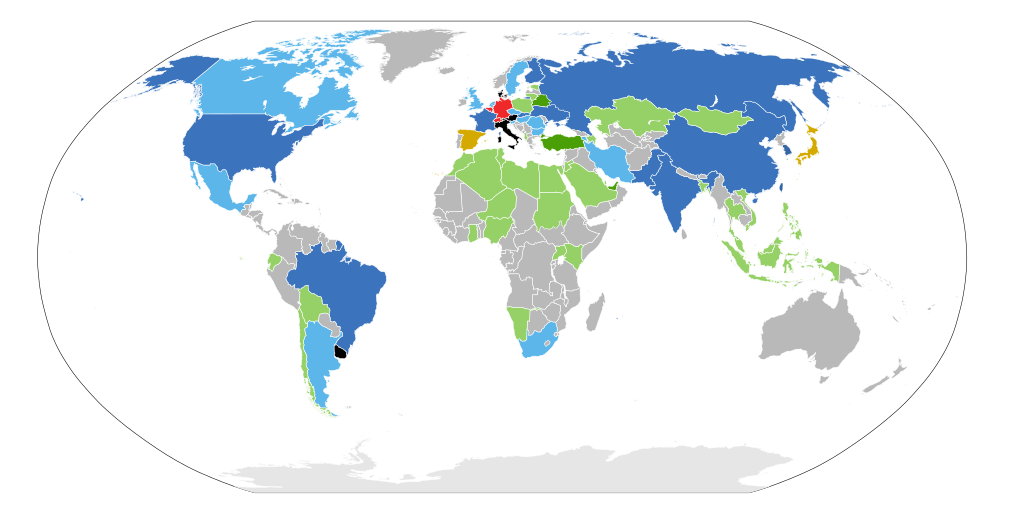
\includegraphics[width=\textwidth]{./images/nuclear-nations-map.png}\\

\vspace{-10mm}
      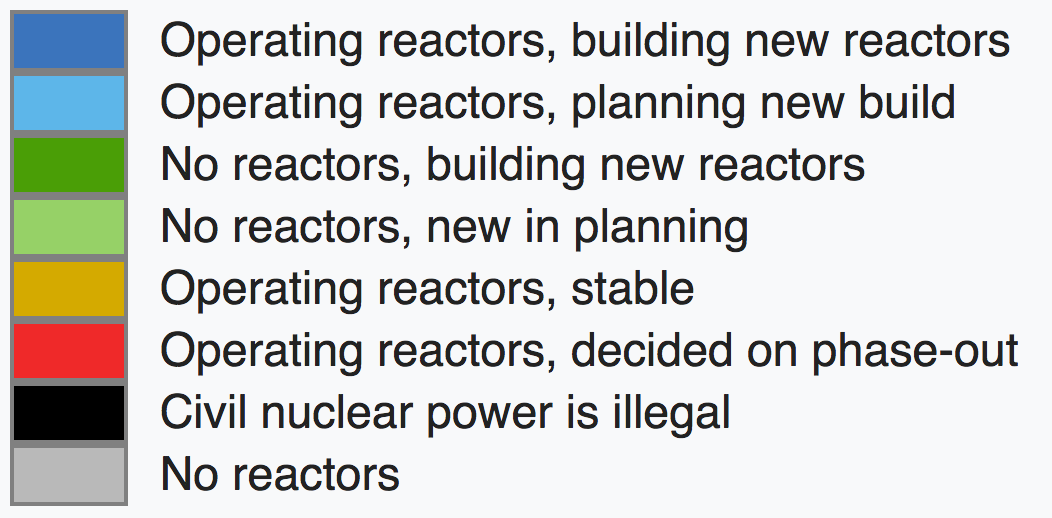
\includegraphics[height=0.2\textheight]{./images/nuclear-nations-legend.png}
    \end{center}
          \caption{Nuclear power status of all nations 
          \cite{paleogene_file:nuclear_2017}.}
    \label{fig:nuc-nations-map}
  \end{figure}
\end{frame}

\begin{frame}
  \frametitle{Nuclear Weapons Nations}
  % a comment
  \begin{figure}[htbp!]
    \begin{center}
      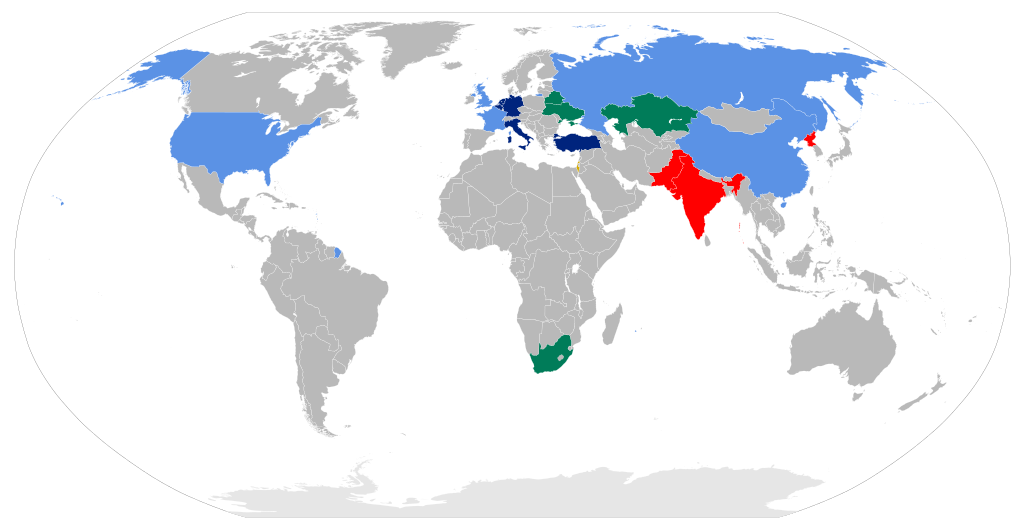
\includegraphics[width=\textwidth]{./images/nuclear-weapons-map.png}\\

\vspace{-10mm}
      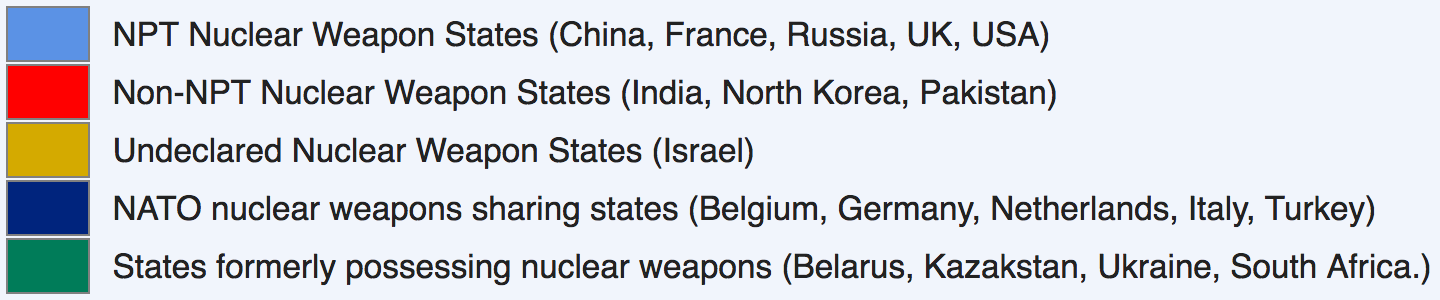
\includegraphics[height=0.2\textheight]{./images/nuclear-weapons-legend.png}
    \end{center}
          \caption{Nuclear power status of all nations 
          \cite{paleogene_file:nuclear_2017}.}
    \label{fig:nuc-nations-map}
  \end{figure}
\end{frame}




\begin{frame}
  \frametitle{Power vs. Weapons}
  % a comment
        \begin{columns}
                \column[t]{0.6\textwidth}
        \begin{center}
      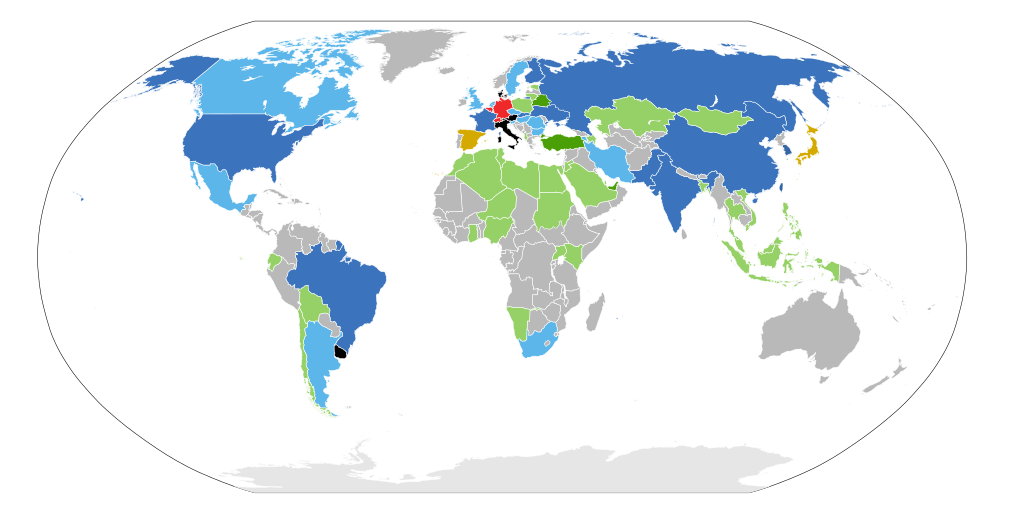
\includegraphics[width=\textwidth]{./images/nuclear-nations-map.png}\\
    \end{center}
                \column[t]{0.6\textwidth}
\hspace{-1in}
                \begin{center}
		      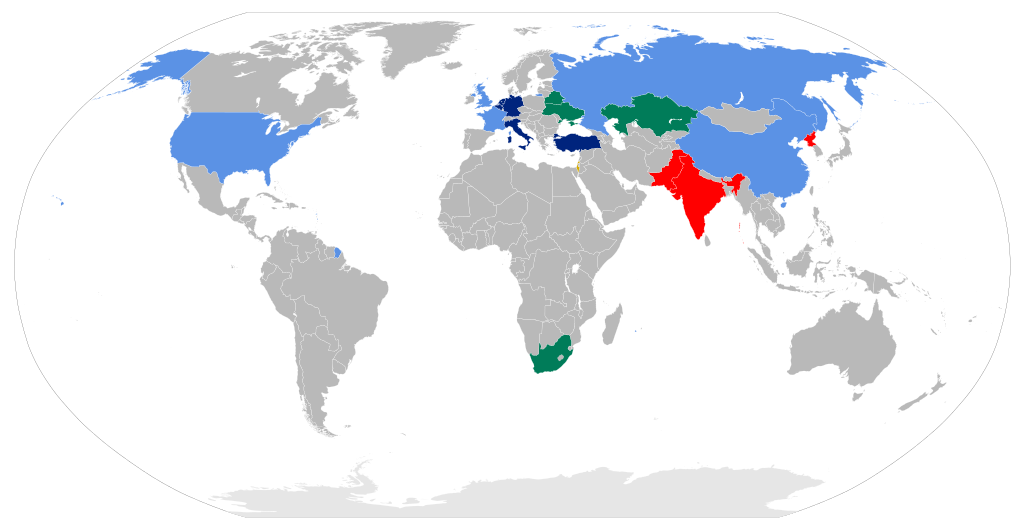
\includegraphics[width=\textwidth]{./images/nuclear-weapons-map.png}
                \end{center}
        \end{columns}
\end{frame}        

\begin{frame}
  \frametitle{International Reactors}
  % a comment
  \begin{figure}[htbp!]
    \begin{center}
      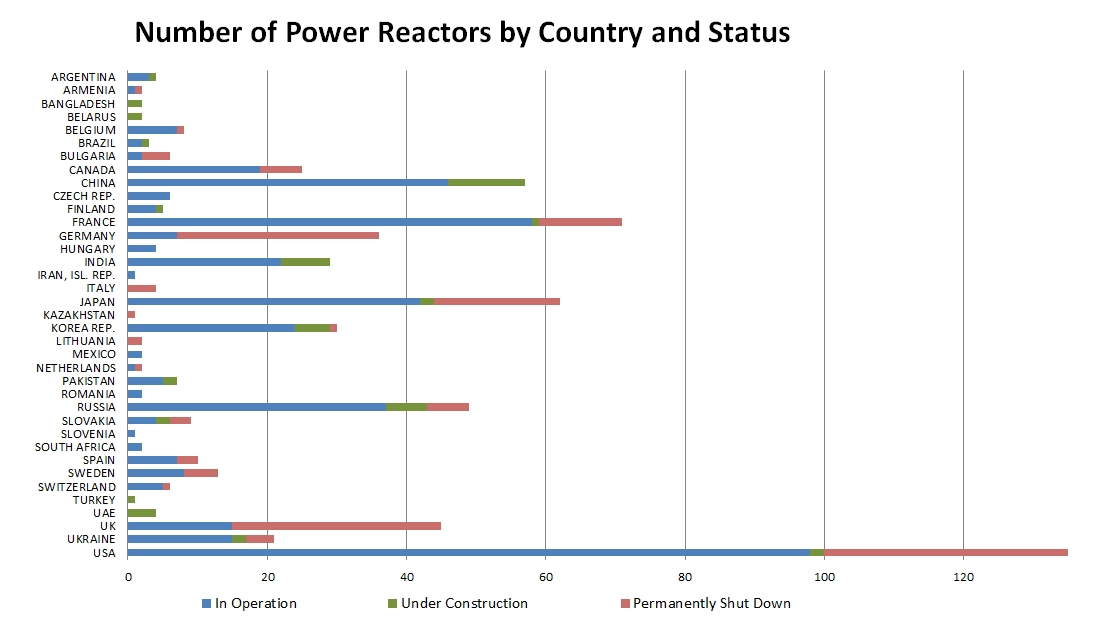
\includegraphics[width=\textwidth]{./images/nuclear-nations.eps}
    \end{center}
          \caption{Nuclear reactors internationally, replicated from 
          \cite{iaea_country_2015}.}
    \label{fig:nuc-nations}
  \end{figure}
\end{frame}

\begin{frame}
  \frametitle{Nuclear Capacity}
  \begin{figure}[htbp!]
    \begin{center}
      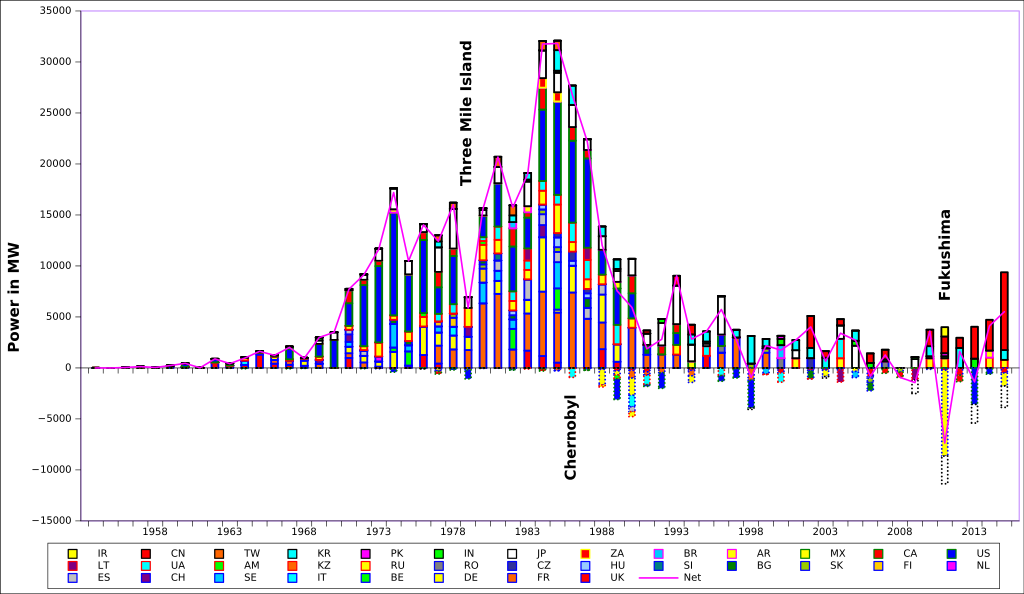
\includegraphics[width=0.9\textwidth]{./images/nuclear-nations-deployments.png}
    \end{center}
          \caption{Nuclear power deployments as a function of time
          \cite{torsch_global_2013}.}
    \label{fig:nuc-nations-deployments}
\end{figure}
\end{frame}


\subsection{Spent Fuel Inventory}
\begin{frame}[fragile]
        \frametitle{Spent Fuel Inventory}
\begin{block}{High Level Waste}
        \begin{itemize}
                \item 270,000 metric tons worldwide
                \item 90\% in storage pools 
                \item remainder in dry casks
        \end{itemize}
                
\includegraphics[height=0.2\textheight]{./images/catinhat}
        \end{block}
\end{frame}

\begin{frame}[fragile]
        \frametitle{Spent Fuel Inventory}
    \begin{table}
      \centering
      \footnotesize{
      \begin{tabular}{l|lll}
        \multicolumn{4}{c}{\textbf{Radioactive Waste Volumes}}\\
        \hline
Type & In storage ($m^3$) & In disposal ($m^3$)  &  \% in disposal\\
        \hline
VLLW &   2,356,000 &   7,906,000  &  77\%\\
LLW  &  3,479,000  &  20,451,000 &   85\%\\
ILW  &  460,000  &  107,000  &  19\%\\
HLW  &  22,000 &   0   & 0\%\\
        \hline
      \end{tabular}
      \caption[SNF volumes]{Solid radioactive waste volumes worldwide, IAEA 
      estimate 2016. \cite{iaea}}
      \label{tab:vol}
      }
    \end{table}
    \end{frame}



\section{Spent Fuel Options}

%%--------------------------------%%
\begin{frame}[c]
    \frametitle{Array of Possible Options}
    \begin{figure}[htbp!]
  \begin{center}
    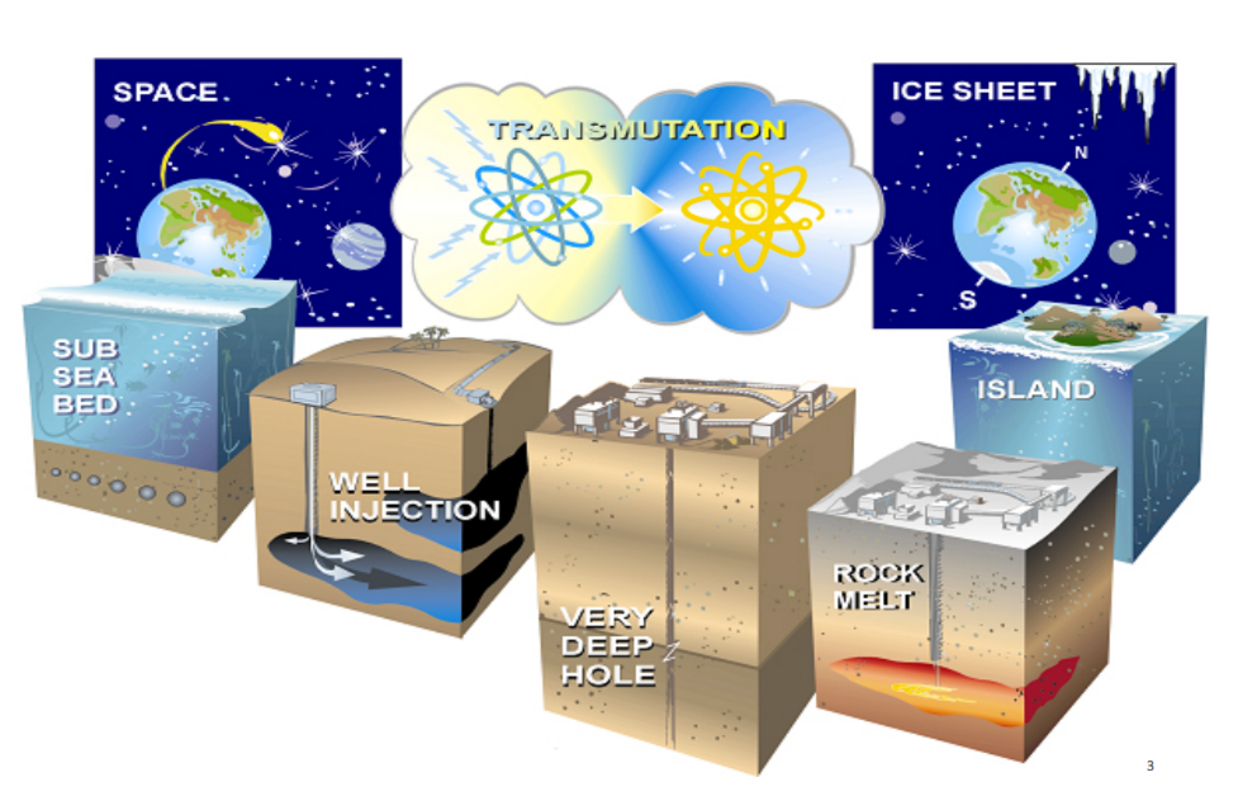
\includegraphics[height=0.7\textheight]{./images/alternative_options.eps}
  \end{center}
  \caption{An array of options have been considered in the past 
    \cite{peters_whats_2013}.}
  \label{fig:alternative_options}
\end{figure}

  \end{frame}

\subsection{Long-Term Storage}

%%--------------------------------%%
\begin{frame}[c]
  \frametitle{Spent Nuclear Fuel}
  \begin{figure}[htb!]
  \begin{center}
    \includegraphics[height=0.7\textheight]{./images/fuel_assembly.eps}
  \end{center}
  \caption{Spent nuclear fuel from conventional power reactors is in the form of
    uranium oxide fuel rods \cite{nrc_nuclear-fuel.jpg_nodate}.}
  \label{fig:snf}
\end{figure}

\end{frame}

\begin{frame}[fragile]
        \frametitle{VLLW, LLW, ILW}
                

  \begin{figure}[htbp!]
    \begin{center}
    \begin{minipage}[t]{0.44\textwidth}
      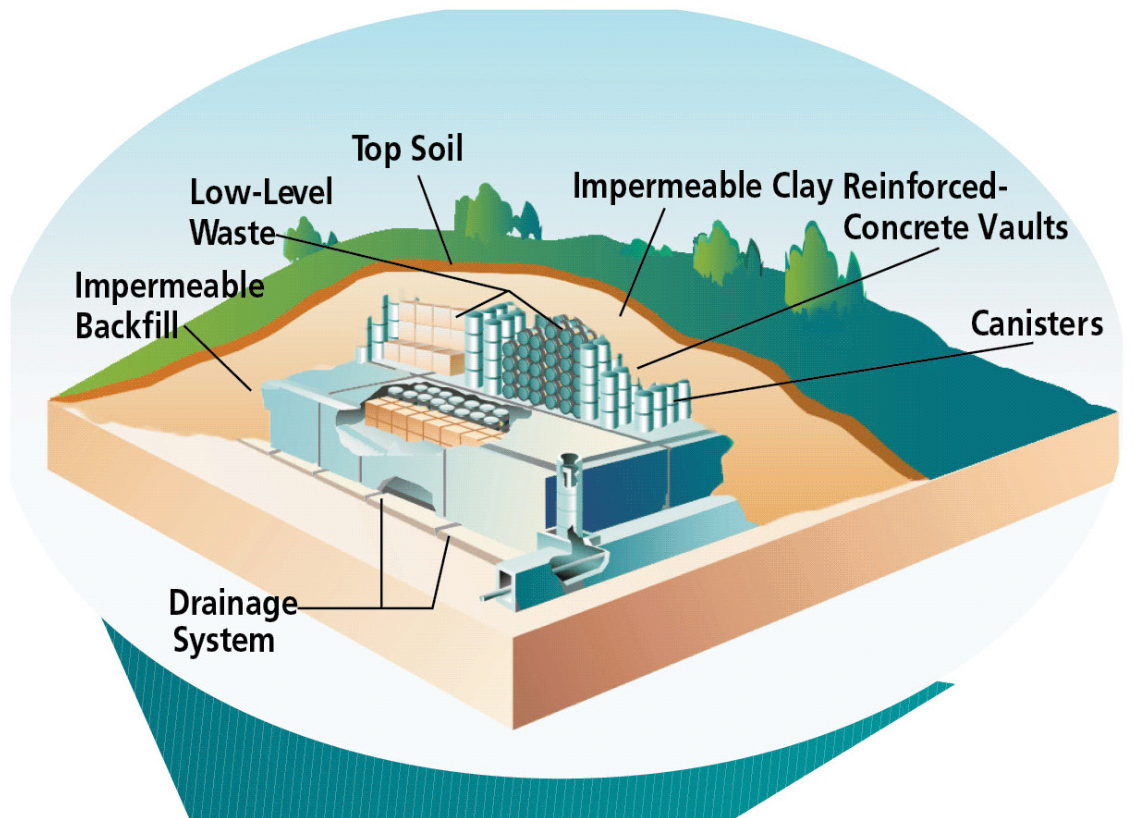
\includegraphics[width=\textwidth]{./images/llw-disposal-cartoon}
      \caption{Design of a LLW repository.}
        \label{fig:llw-cartoon}
    \end{minipage}
    \hspace{0.01\textwidth}
    \begin{minipage}[t]{0.44\textwidth}
      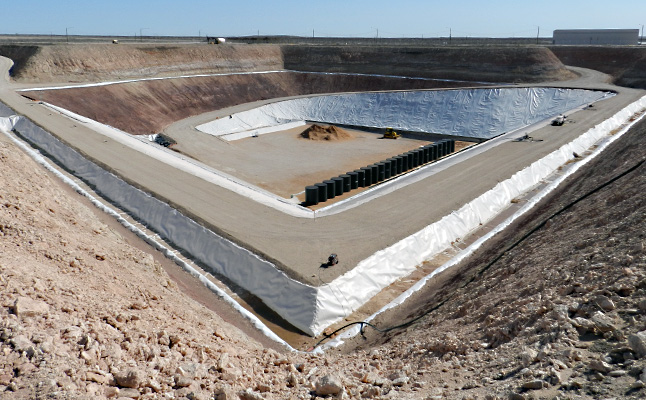
\includegraphics[width=\textwidth]{./images/wcs-andrews-tx.png}
      \caption{Waste Control Specialists Low Level Waste Repository in Andrews 
            County, Tx.}
        \label{fig:wcs}
    \end{minipage}
    \end{center}
  \end{figure}



\end{frame}

\begin{frame}[fragile]
        \frametitle{Spent Fuel Inventory}
                \begin{figure}[htb!]
  \begin{center}
    \includegraphics[height=0.7\textheight]{./images/fuel_assembly.eps}
  \end{center}
  \caption{Spent nuclear fuel from conventional power reactors is in the form of
    uranium oxide fuel rods \cite{nrc_nuclear-fuel.jpg_nodate}.}
  \label{fig:snf}
\end{figure}

\end{frame}

\begin{frame}[fragile]
        \frametitle{Spent Fuel}
        \begin{figure}
        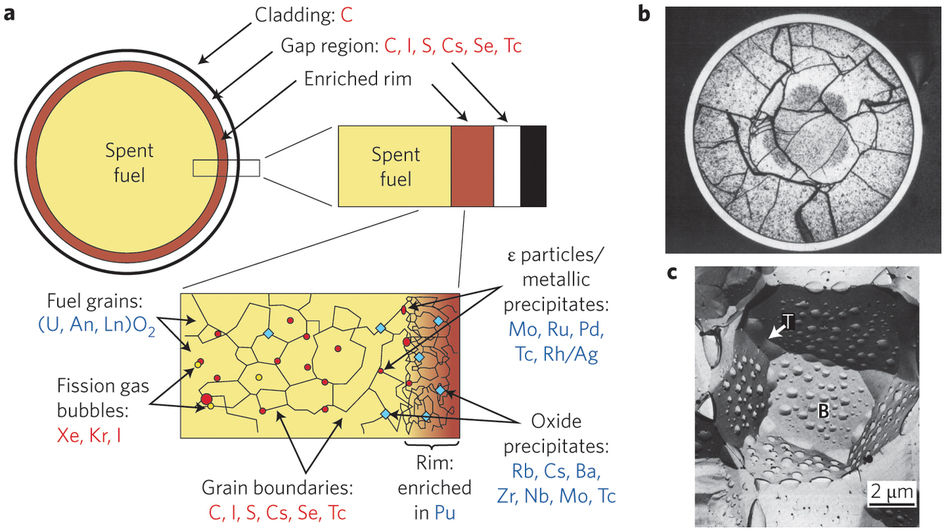
\includegraphics[width=\textwidth]{./images/ewing-microstructure}
                \caption{Microstructure of spent fuel and the distribution of
                fission products and actinides after irradiation in a reactor.
                From \cite{ewing_long-term_2016}.}
        \end{figure}
\end{frame}

\begin{frame}[fragile]
        \frametitle{Spent Fuel Inventory}
                

  \begin{figure}[htbp!]
    \begin{center}
    \begin{minipage}[t]{0.45\textwidth}
      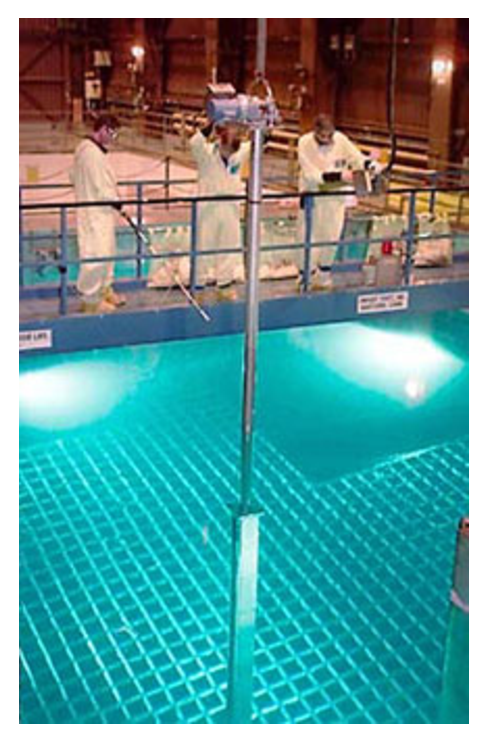
\includegraphics[height=0.4\textheight]{./images/pool.eps}
      \caption{Spent fuel pools are at reactor sites and elsewhere 
        \cite{doe_spent_????}.}
        \label{fig:pool}
    \end{minipage}
    \hspace{0.01\textwidth}
    \begin{minipage}[t]{0.45\textwidth}
      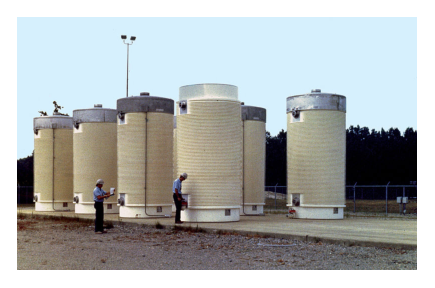
\includegraphics[height=0.4\textheight]{./images/casks.eps}
      \caption{Dry casks at reactor sites and elsewhere \cite{nrc_dry_2008}}
        \label{fig:casks}
    \end{minipage}
    \end{center}
  \end{figure}

\end{frame}


\begin{frame}[fragile]
        \frametitle{Reprocessing Waste}
                \begin{figure}[htbp!]
  \begin{center}
    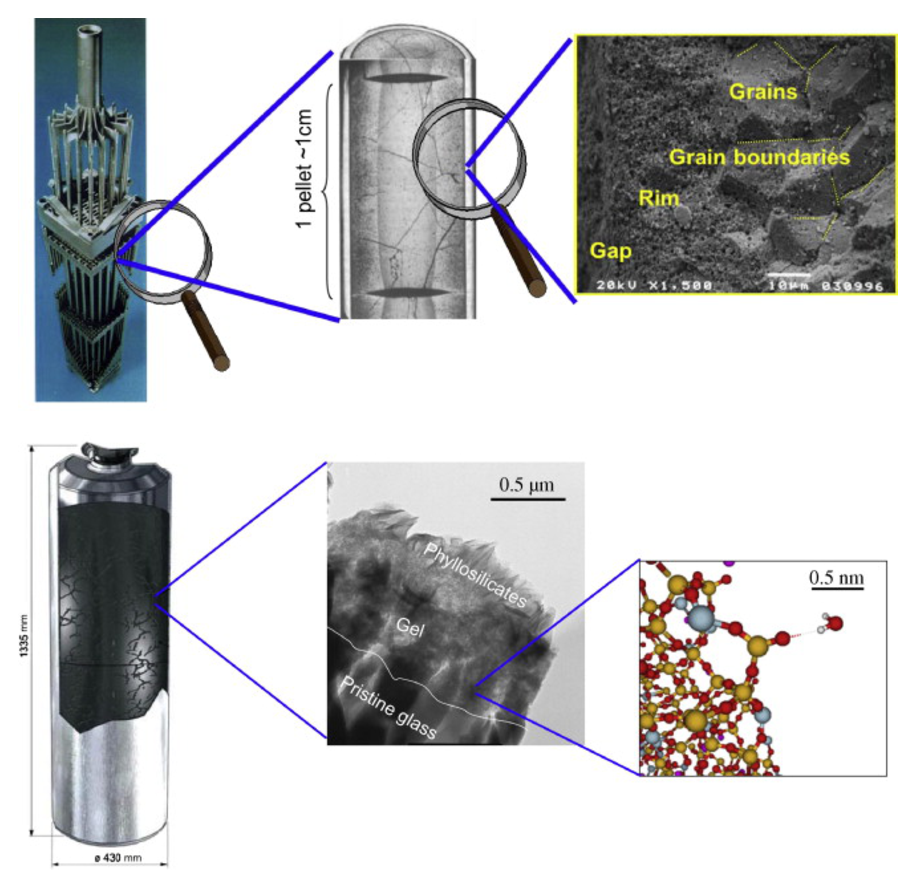
\includegraphics[width=0.5\textwidth]{./images/waste_forms_poinssot.eps}
  \end{center}
  \caption{A comparison of uranium oxide and borosilicate glass waste forms 
  \cite{poinssot_long-term_2012}.}
  \label{fig:waste_forms_poinssot}
\end{figure}

\end{frame}

\begin{frame}[fragile]
        \frametitle{Reprocessing Waste}
                

  \begin{figure}[htbp!]
    \begin{center}
    \begin{minipage}[t]{0.45\textwidth}
      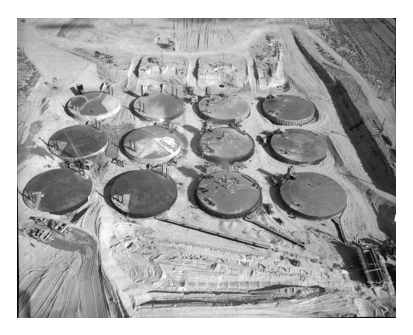
\includegraphics[height=0.4\textheight]{./images/tanks.eps}
        \caption{Liquid waste in steel or carbon steel tanks at Hanford and 
          elsewhere\cite{doe_underground_????}.}
        \label{fig:tanks}
    \end{minipage}
    \hspace{0.01\textwidth}
    \begin{minipage}[t]{0.45\textwidth}
      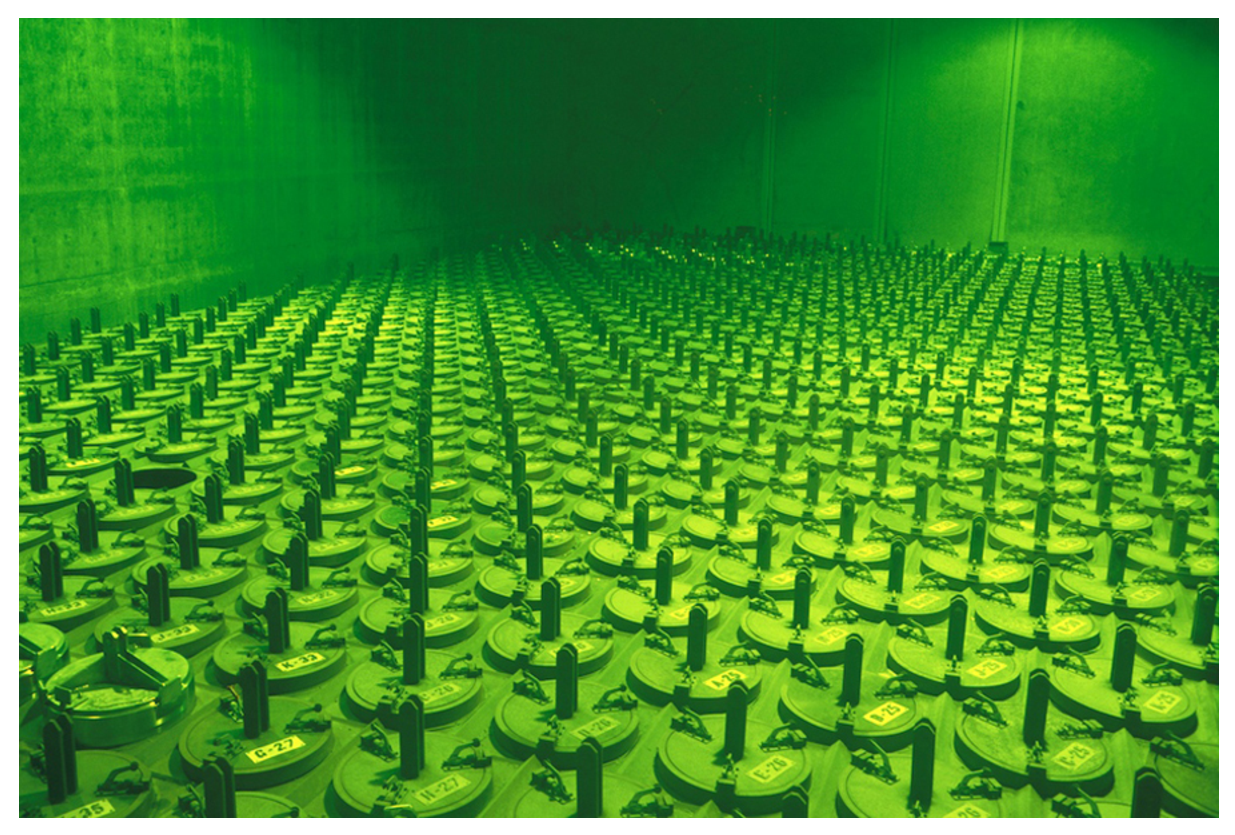
\includegraphics[height=0.4\textheight]{./images/logs.eps}
        \caption{Vitrified glass logs at reprocessing facilities and elsewhere 
          \cite{essick_photographing_2012}.}
        \label{fig:logs}
    \end{minipage}
    \end{center}
  \end{figure}

\end{frame}


\subsection{Reprocessing}

\begin{frame}
  \frametitle{Reprocessing Capacity}
  % a comment
  The reprocessing capacity globally is shown in Fig. \ref{fig:reprocessing-nn}.
  \begin{figure}[htbp!]
    \begin{center}
      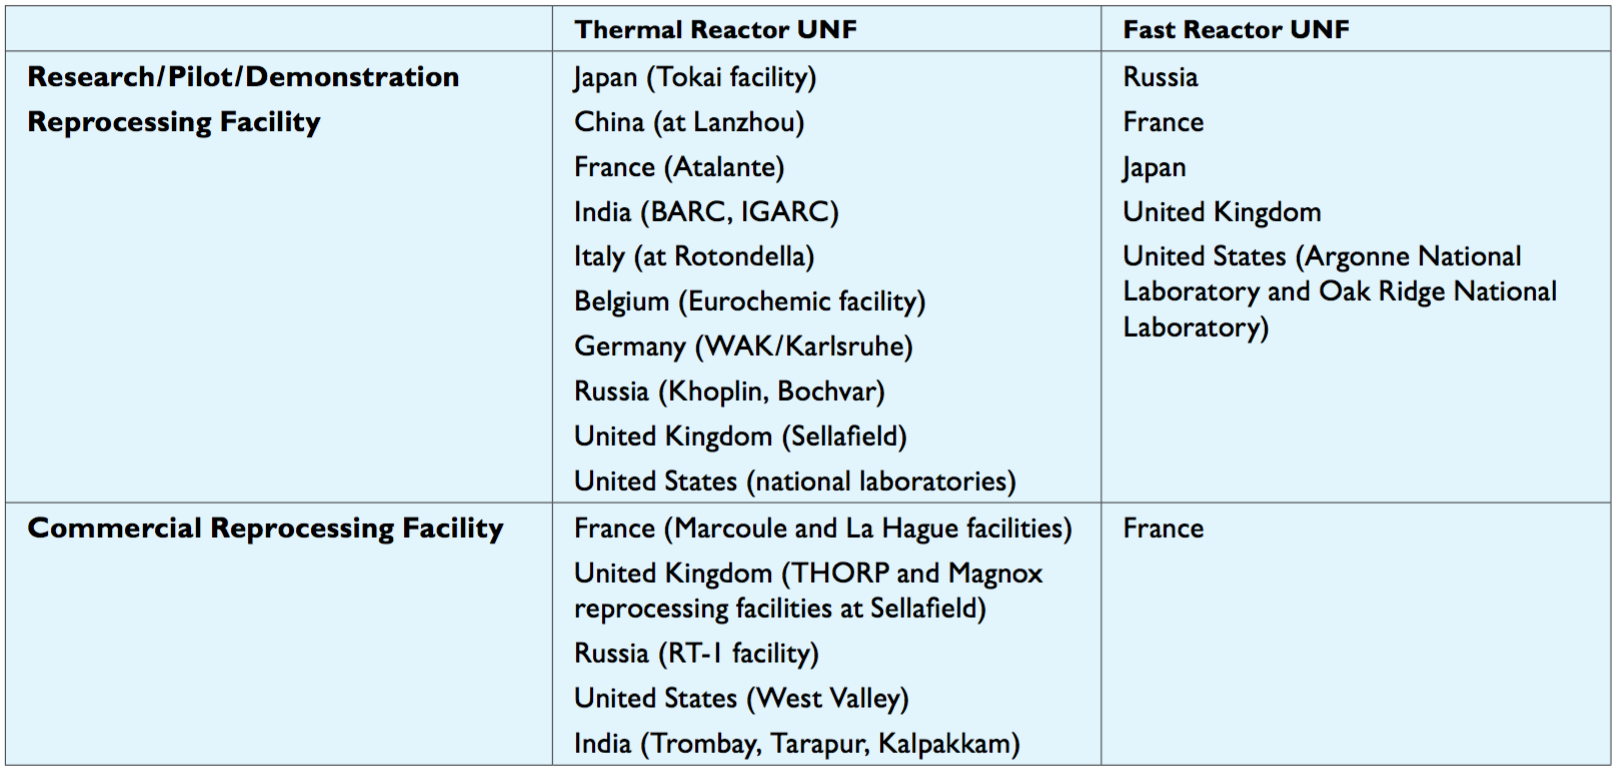
\includegraphics[width=\textwidth]{./images/reprocessing-nn}
    \end{center}
          \caption{\cite{buckner_case_2016}.}
    \label{fig:reprocessing-nn}
  \end{figure}
\end{frame}

\begin{frame}
  \frametitle{MOX production}
  % a comment
  The MOX production globally is shown in Fig.
  \ref{fig:mox-production-nn}.
  \begin{figure}[htbp!]
    \begin{center}
      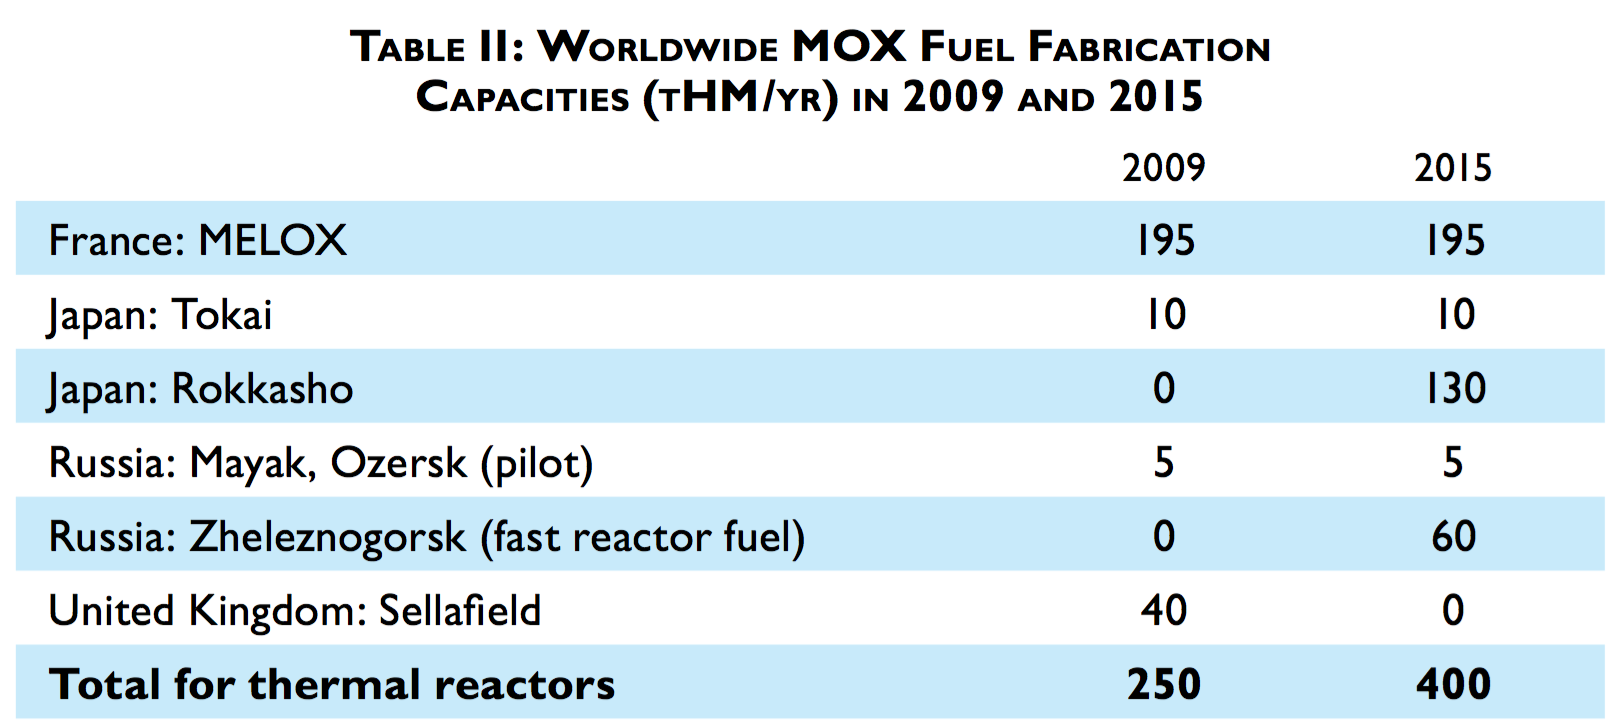
\includegraphics[height=4cm]{./images/mox-production-nn}
    \end{center}
          \caption{\cite{buckner_case_2016}.}
    \label{fig:mox-production-nn}
  \end{figure}
\end{frame}

\subsection{Deep Geologic Disposal}


%%----------------------------------------%%
\begin{frame}
  \frametitle{Repository Components}
\footnotesize{
  \begin{figure}[htbp!]
  \begin{center}
    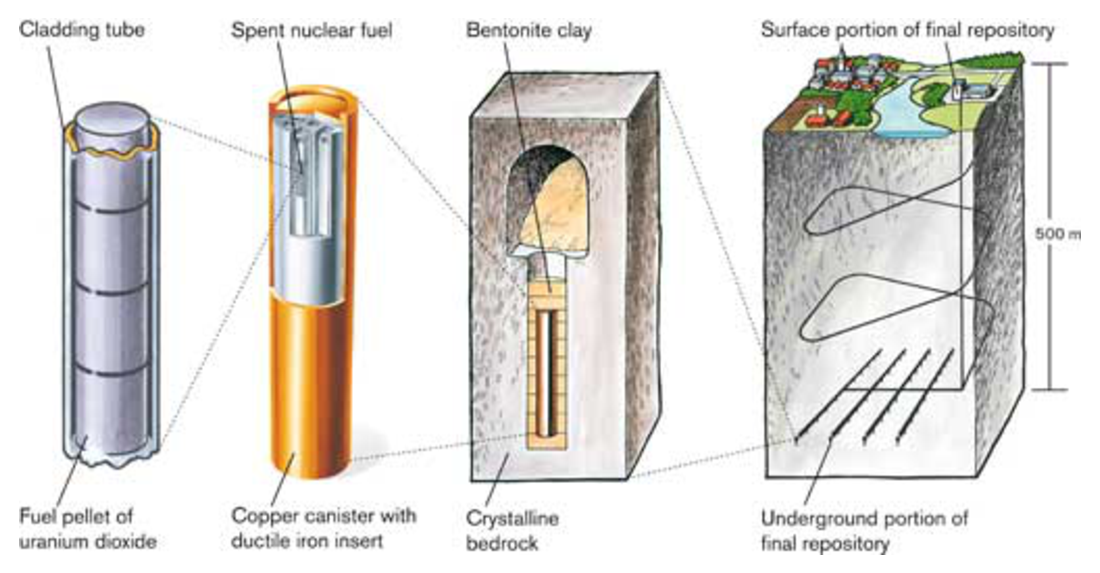
\includegraphics[width=0.7\textwidth]{./images/skb_components.eps}
  \end{center}
  \caption{Geologic disposal systems typically employ engineered barrier 
    systems as well as natural barrier systems. This is a Swedish concept in 
    granite \cite{ab_long-term_2006}.}
  \label{fig:skb_components}
\end{figure}

}
\end{frame}


\begin{frame}
  \frametitle{Repository Layouts}

  \begin{minipage}{0.49\textwidth}
    \begin{figure}[h!]
      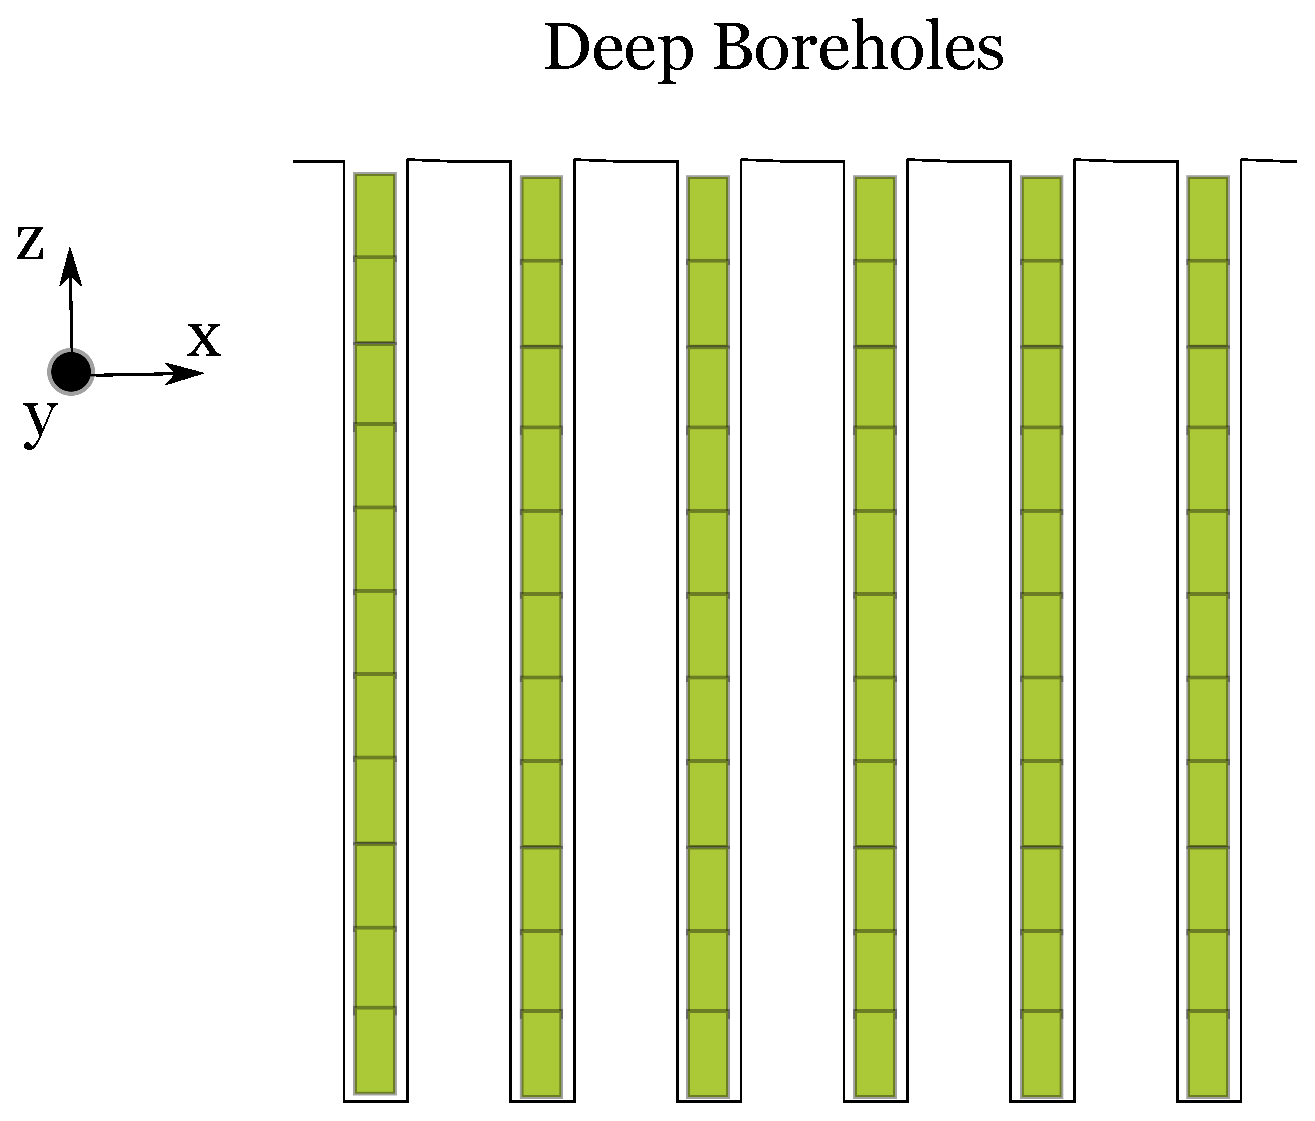
\includegraphics[width=0.75\textwidth]{./images/boreholes.eps}
    \end{figure}
    \begin{figure}[h!]
      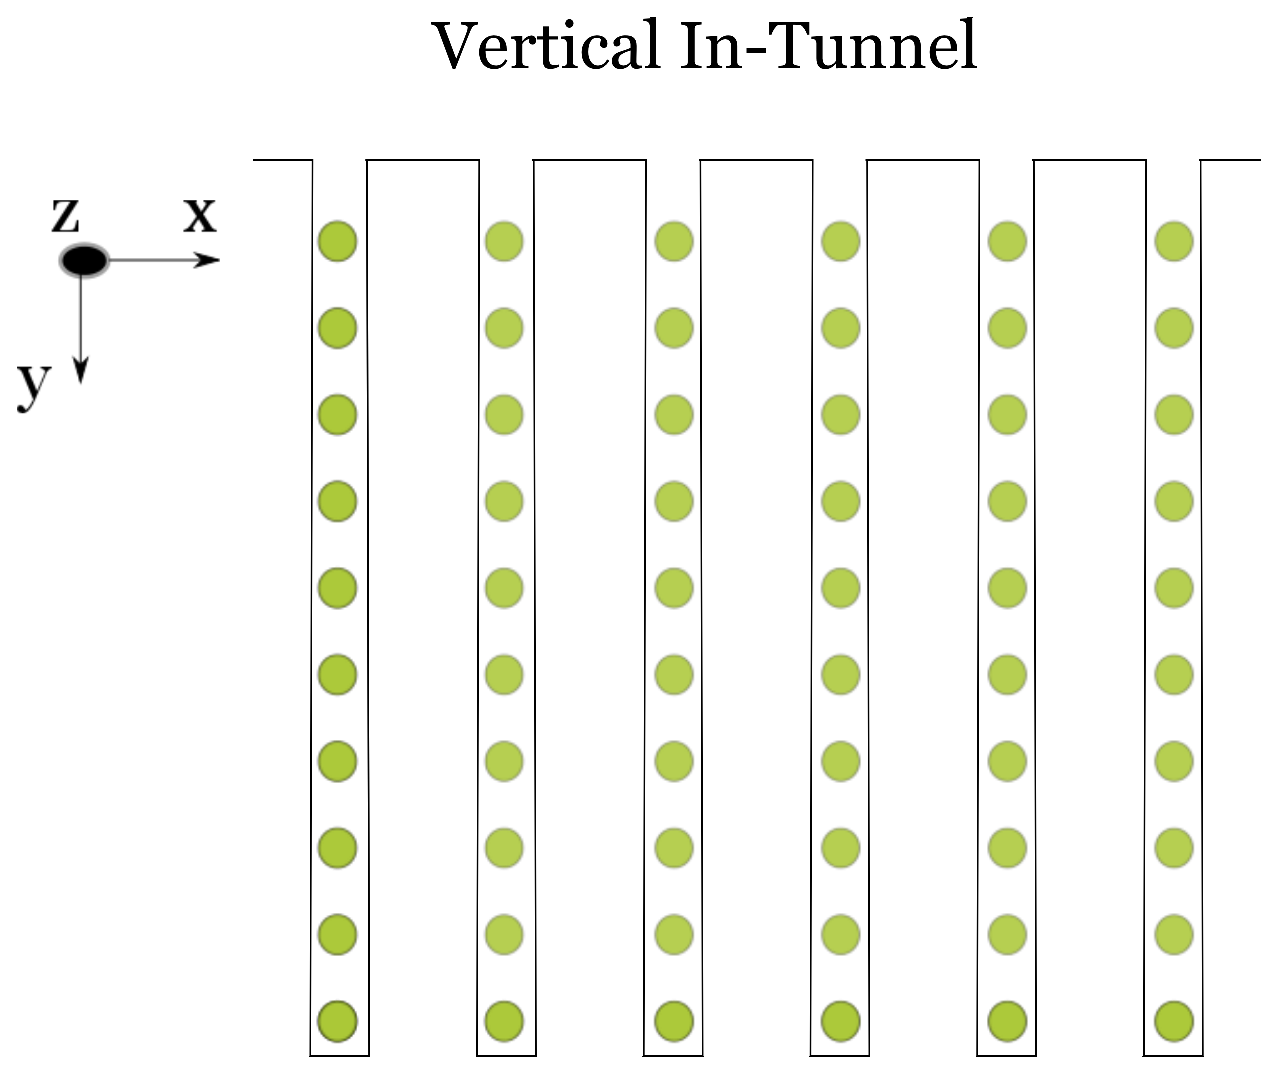
\includegraphics[width=0.75\textwidth]{./images/vertical.eps}
    \end{figure}
  \end{minipage}
  \hspace{0.01cm}
  \begin{minipage}{0.49\textwidth}
    \begin{figure}[h!]
      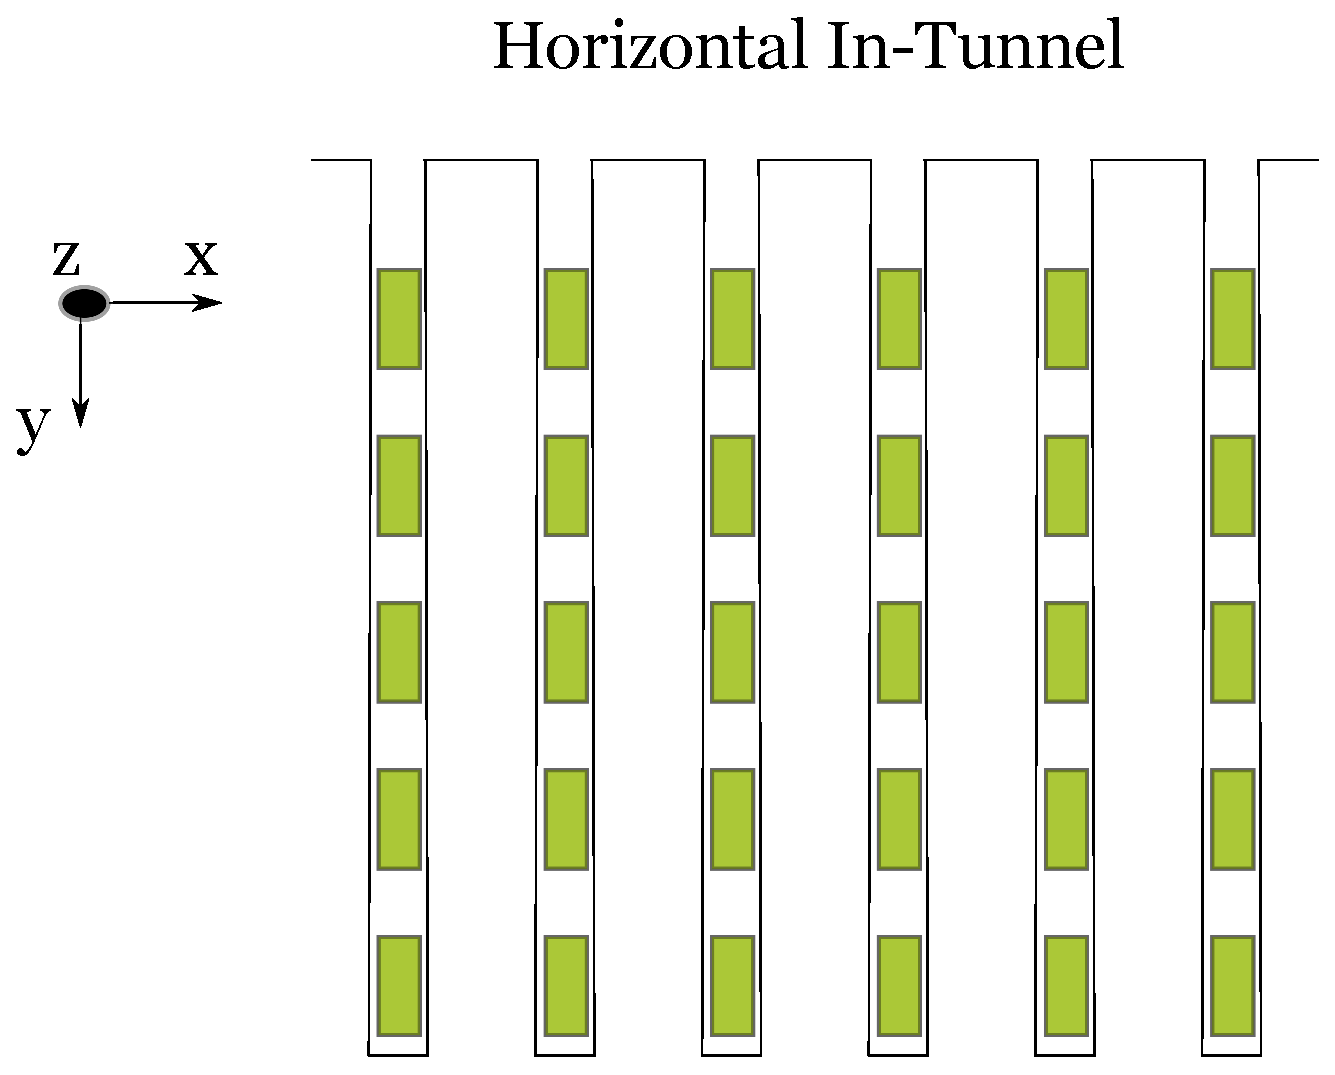
\includegraphics[width=0.8\textwidth]{./images/horizontal.eps}
    \end{figure}
    \begin{figure}[h!]
      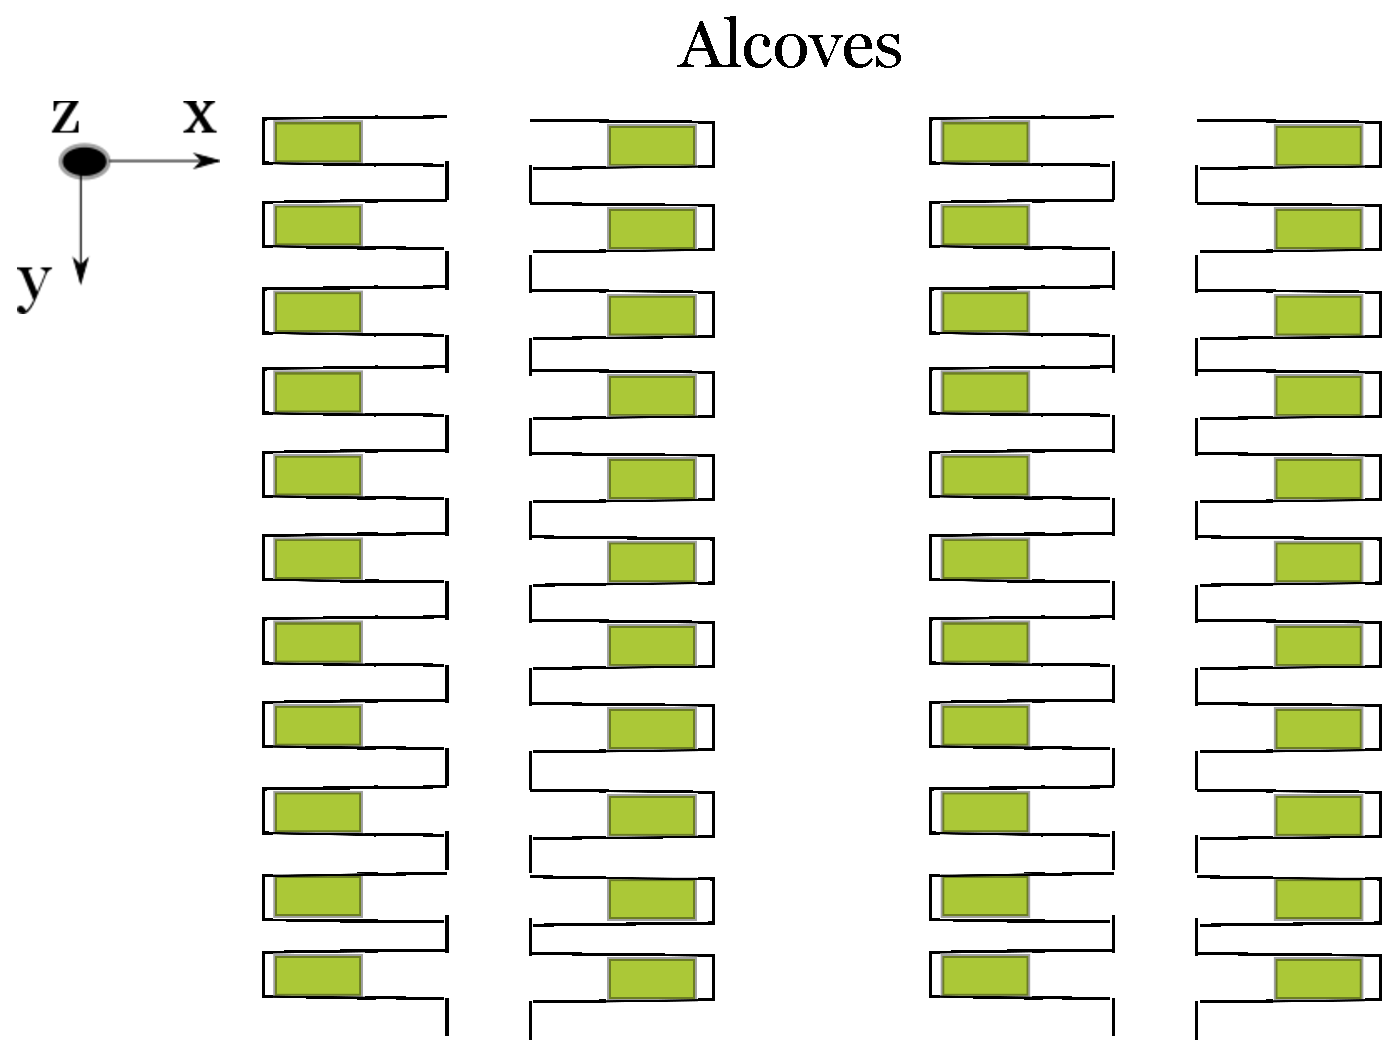
\includegraphics[width=0.8\textwidth]{./images/alcoves.eps}
    \end{figure}
  \end{minipage}

\end{frame}

\begin{frame}
  \footnotesize{
  \frametitle{Unsaturated, Ventilated Concepts}
  \begin{figure}[htbp!]
  \begin{center}
    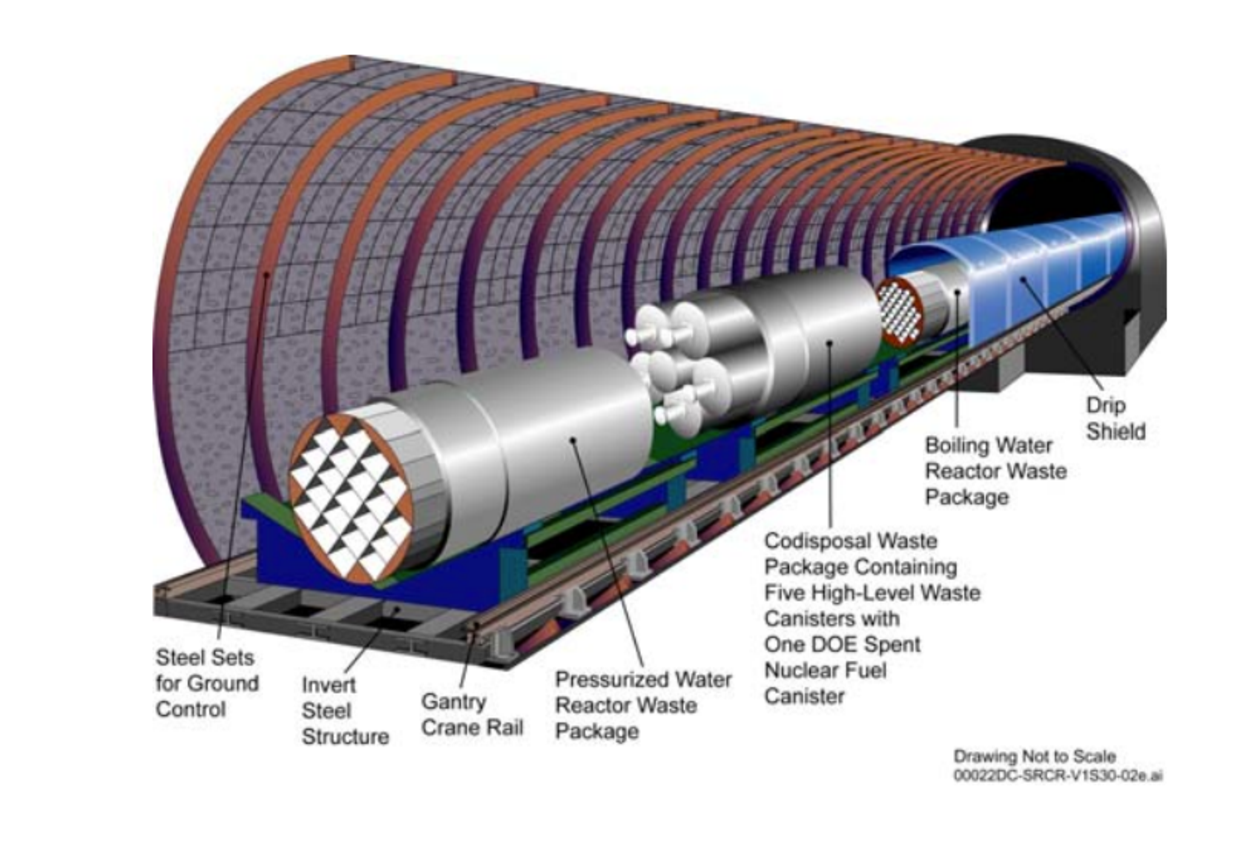
\includegraphics[height=0.7\textwidth]{./images/yucca_tunnel.eps}
  \end{center}
  \caption{The current U.S. geologic disposal concept \cite{peters_whats_2013}.}
  \label{fig:yucca_tunnel}
\end{figure}

}
\end{frame}

\begin{frame}
  \footnotesize{
  \frametitle{Saturated , Enclosed Concepts} 
 \begin{figure}[h!]
    \begin{center}
      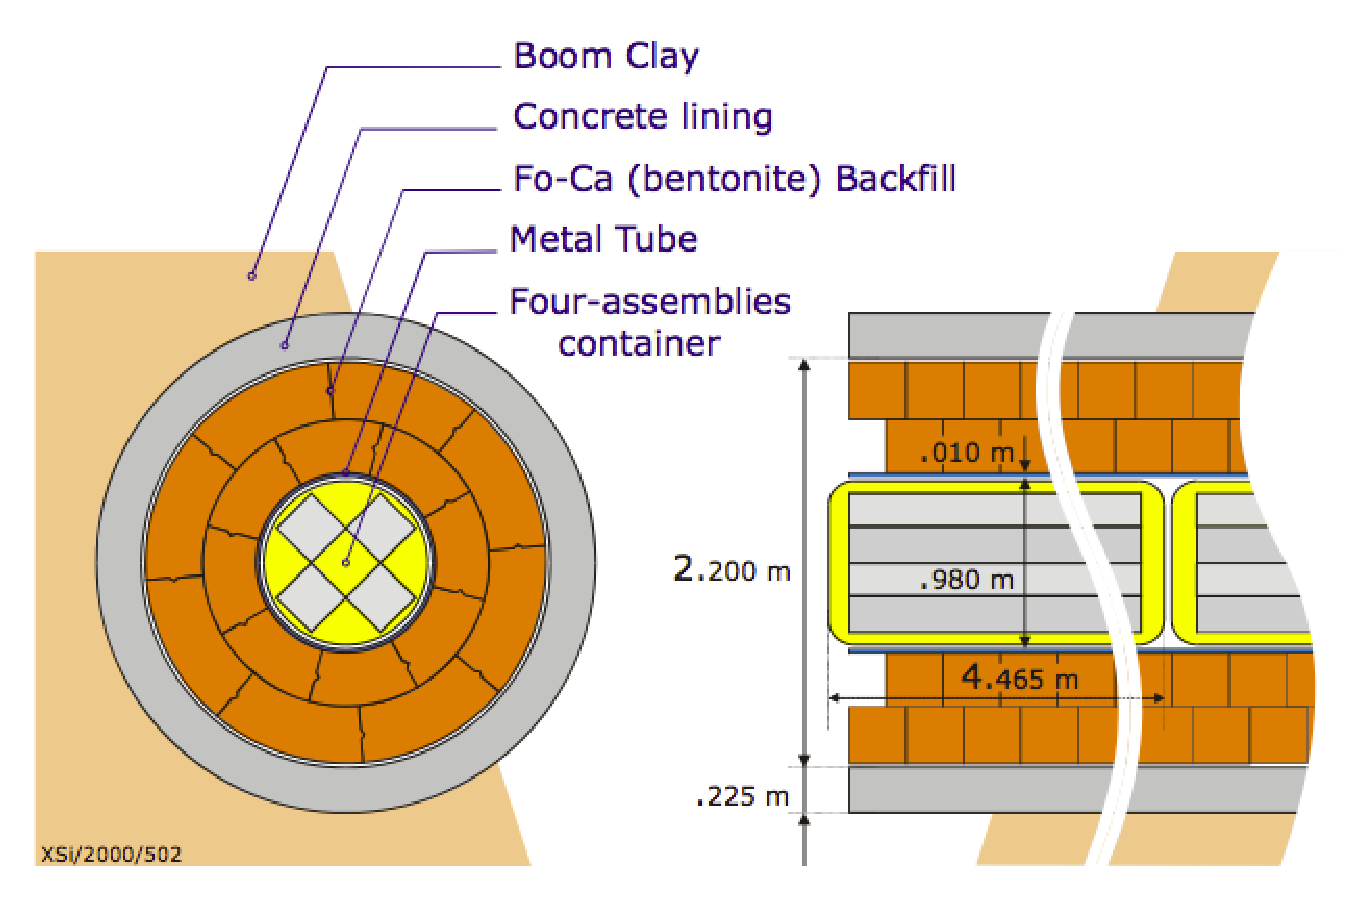
\includegraphics[height=.7\textheight]{./images/belgianClayRedImp.eps}
    \end{center}
    \caption{The Belgian reference concept in Boom Clay is backfilled very soon
   after waste emplacement without a ventilation period and is located below the water table
   \cite{von_lensa_red-impact_2008}.}
    \label{fig:belgianClayRedImp}
  \end{figure}
}
\end{frame}



\begin{frame}
  \frametitle{Tuff (Yucca) Disposal Environments}
  \footnotesize{
    \begin{figure}[htbp!]
  \begin{center}
    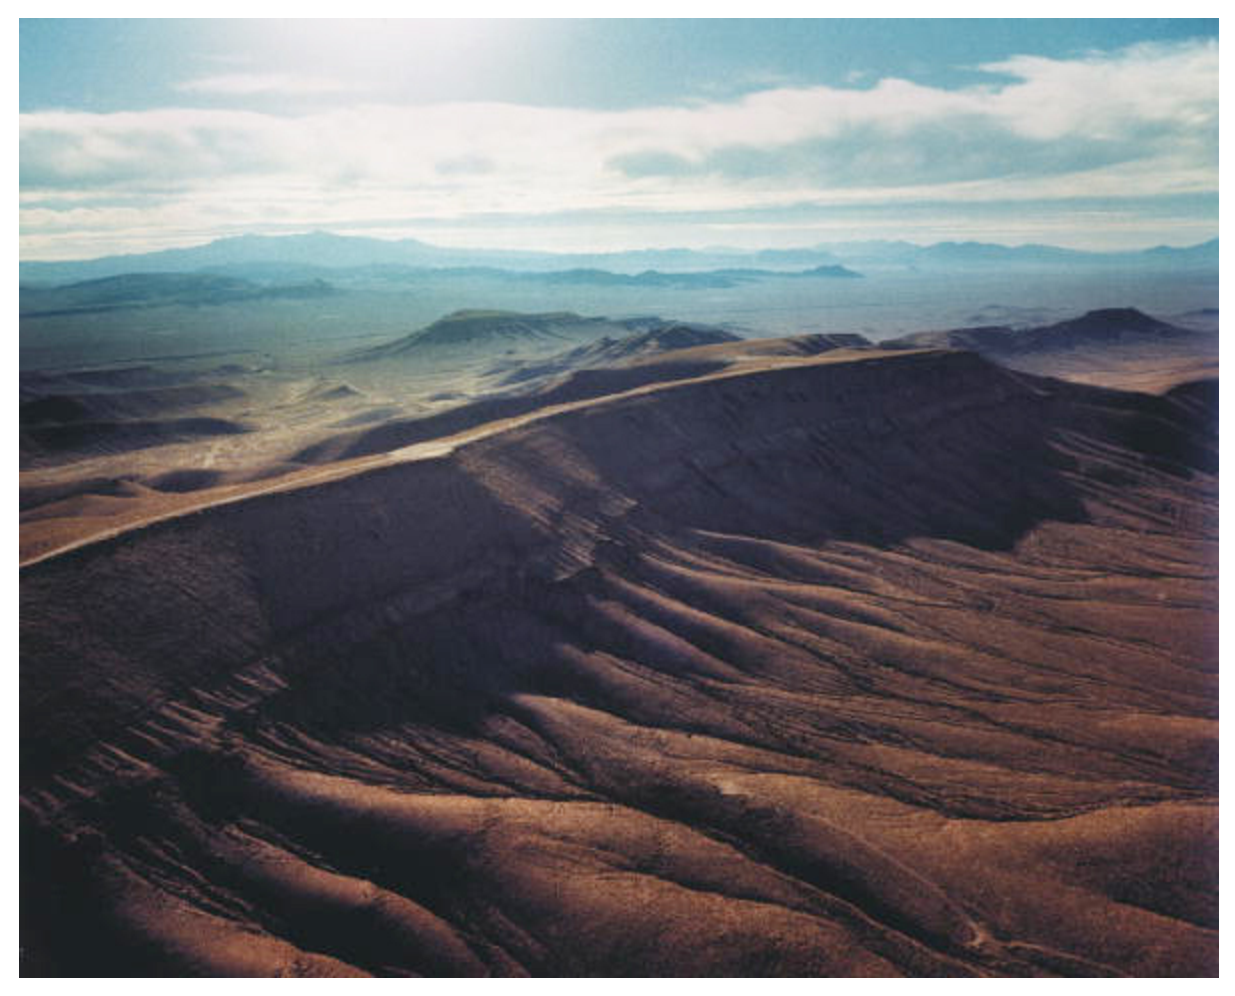
\includegraphics[width=0.5\textwidth]{./images/yucca_site.eps}
  \end{center}
  \caption{Yucca Mountain is in southern Nevada \cite{omb_yucca_2006}.}
  \label{fig:yucca_site}
\end{figure}

  }
\end{frame}

\begin{frame}
  \frametitle{Alternative Disposal Geology Options}
   \begin{minipage}{0.44\textwidth}
     \begin{figure}[h!]
         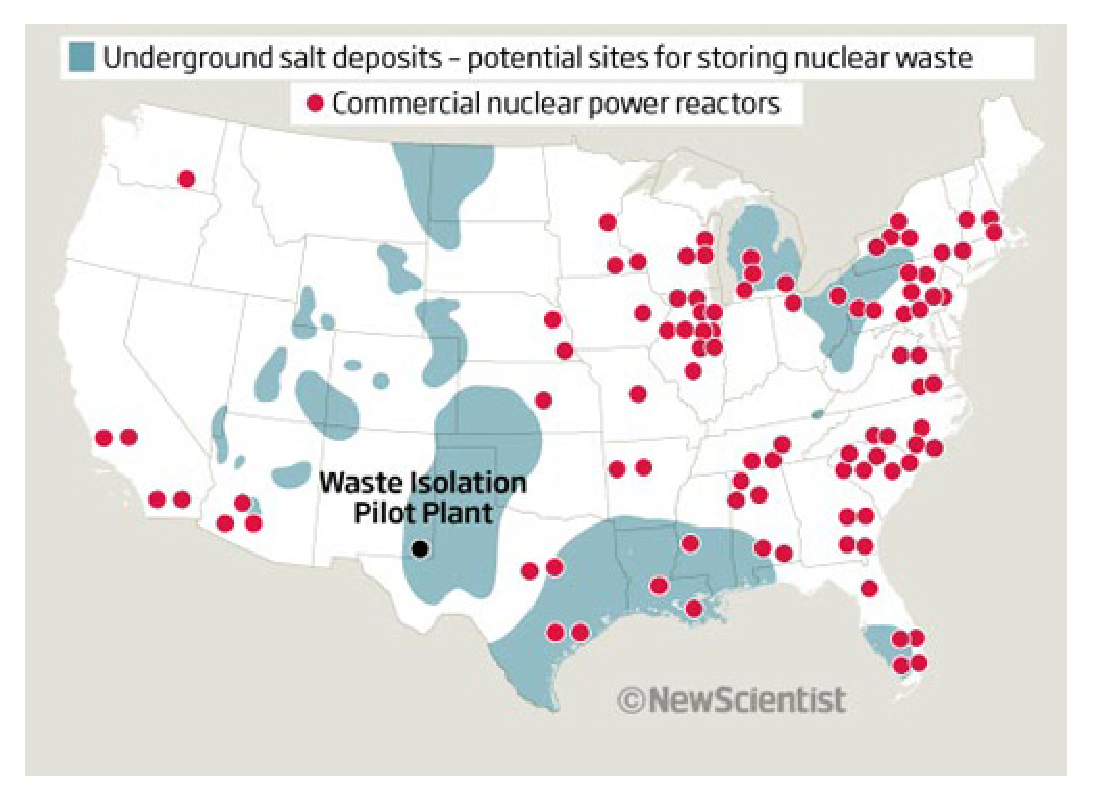
\includegraphics[width=0.8\textwidth]{./images/saltNewScientist.eps}
         \caption{U.S. Salt Deposits, ref. \cite{newscientist_where_2011}.}
     \end{figure}
     \begin{figure}[h!]
         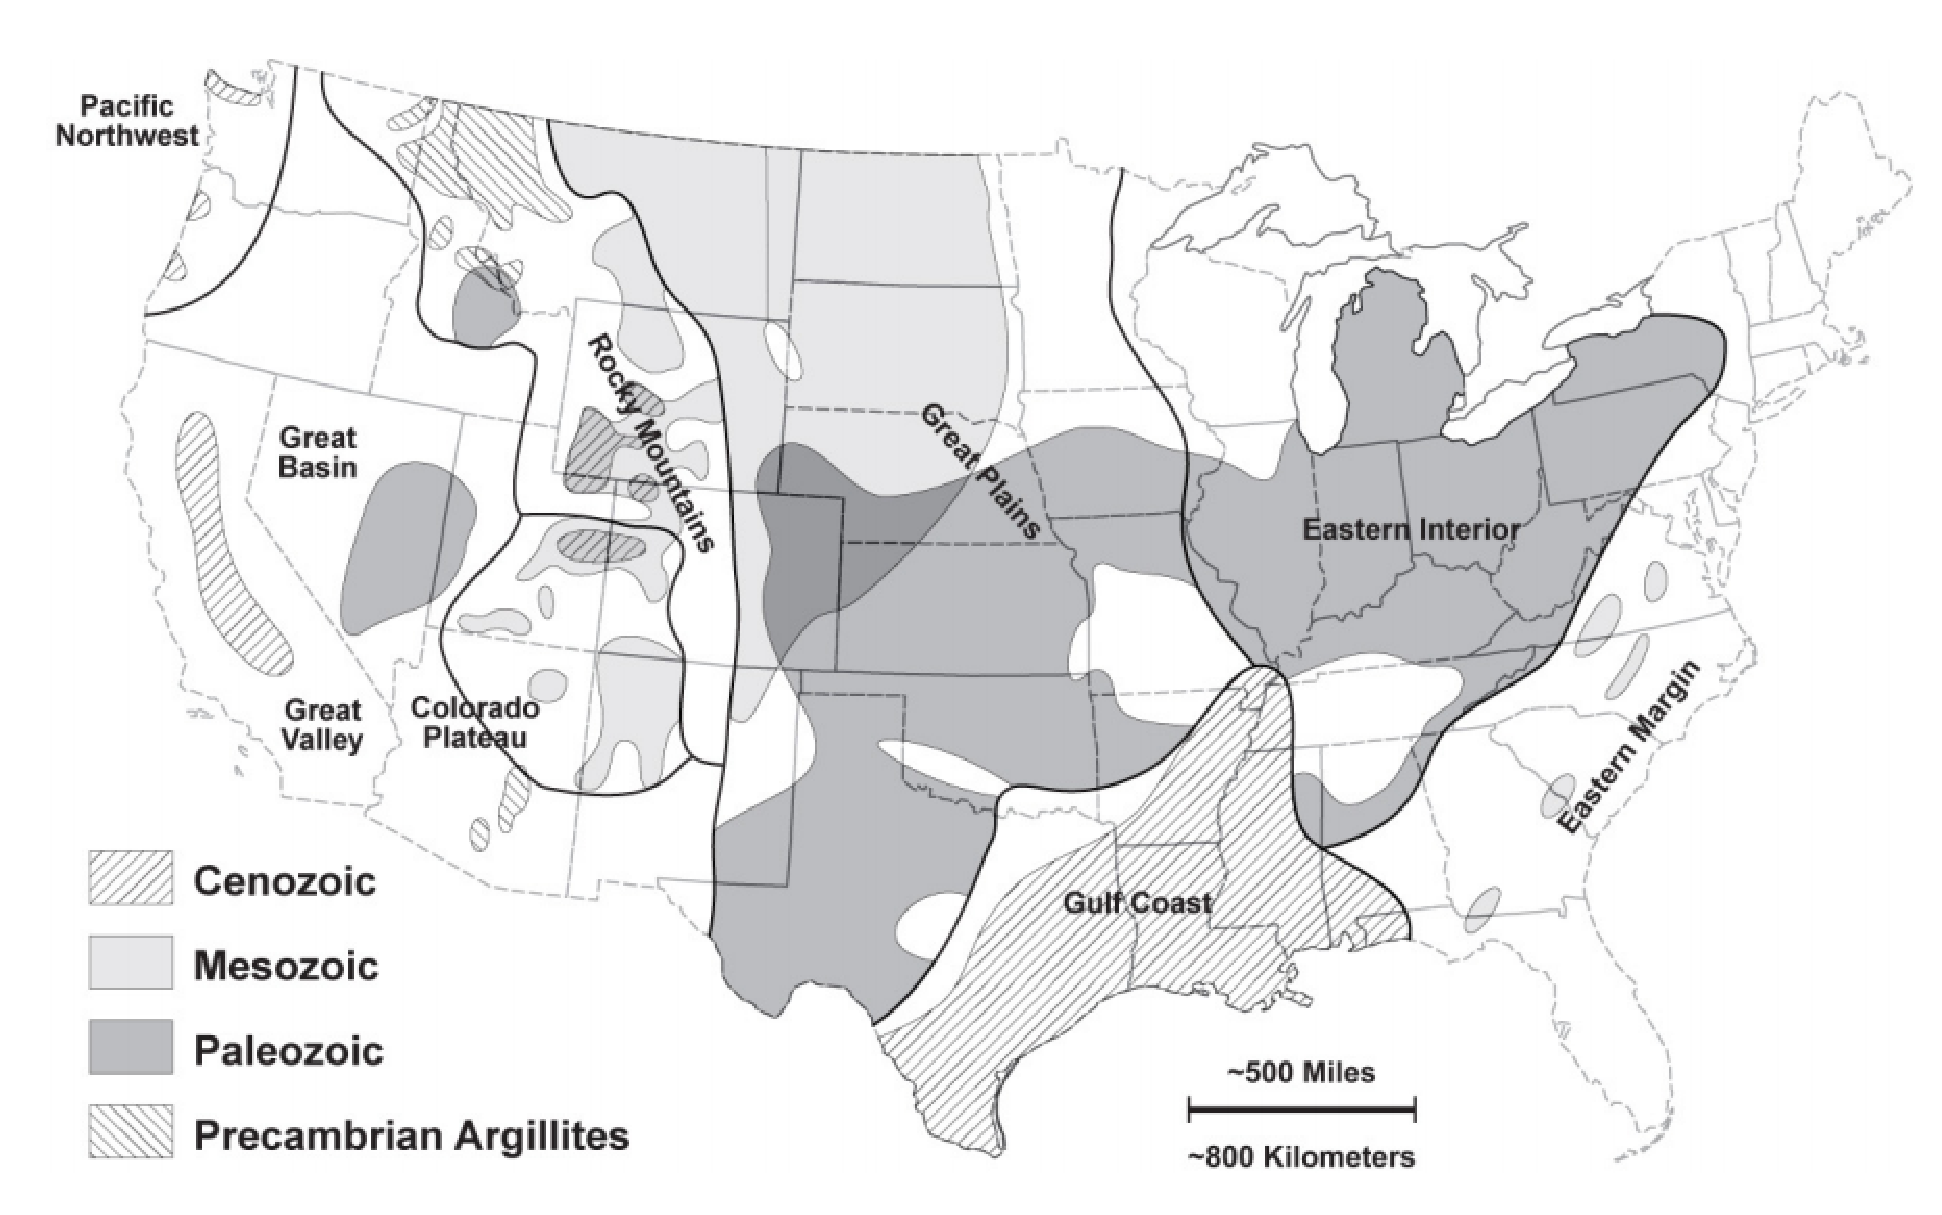
\includegraphics[width=0.8\textwidth]{./images/clayGonzales.eps}
         \caption{U.S. Clay Deposits, ref. \cite{gonzales_shales_1985}.}
     \end{figure}
   \end{minipage}
   \hspace{0.01cm}
   \begin{minipage}{0.44\textwidth}
     \begin{figure}[h!]
         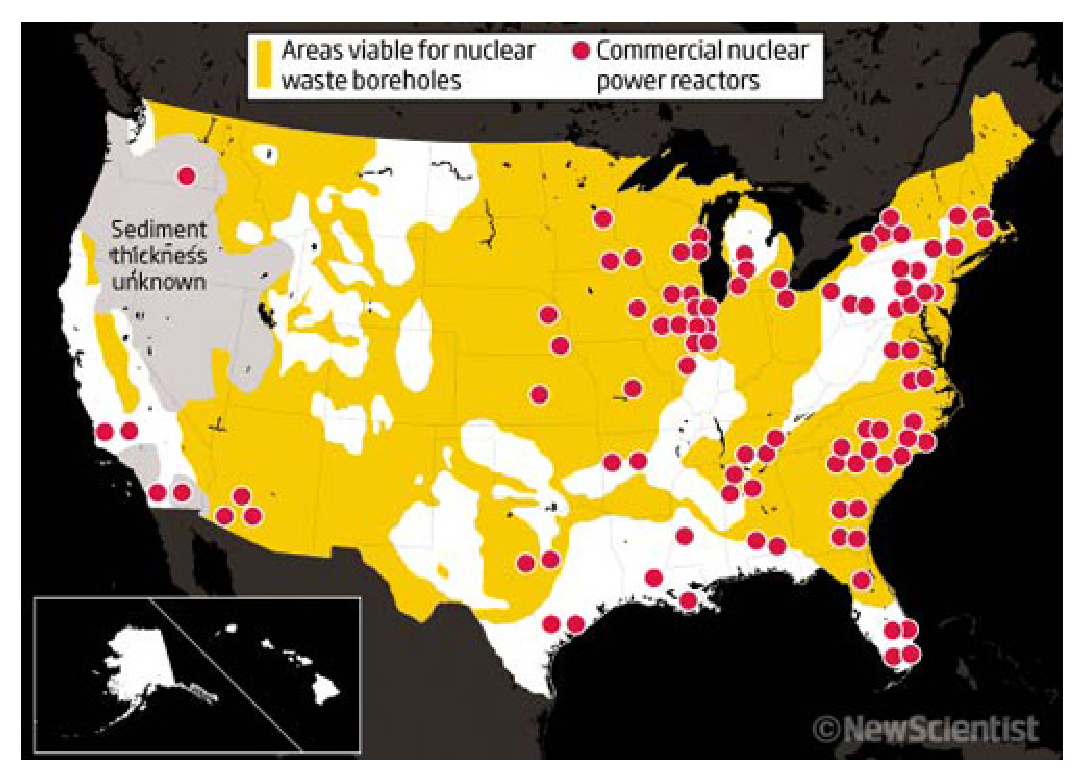
\includegraphics[width=0.8\textwidth]{./images/boreholeNewScientist.eps}
         \caption{U.S. Crystalline Basement, ref.  \cite{newscientist_where_2011}.}
     \end{figure}
     \begin{figure}[h!]
         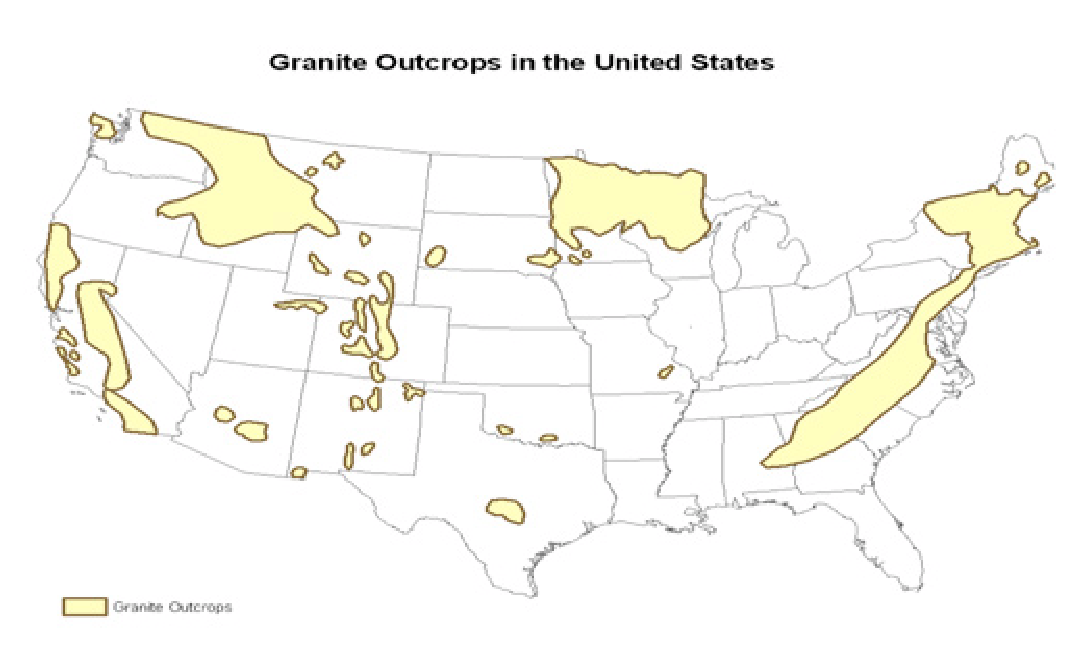
\includegraphics[width=0.8\textwidth]{./images/graniteBush.eps}
         \caption{U.S. Granite Beds, ref. \cite{bush_economic_1976}.}
     \end{figure}
   \end{minipage}
\end{frame}

\begin{frame}
  \frametitle{Clay Disposal Environments}
  \footnotesize{

  \begin{figure}[h!]
    \begin{center}
      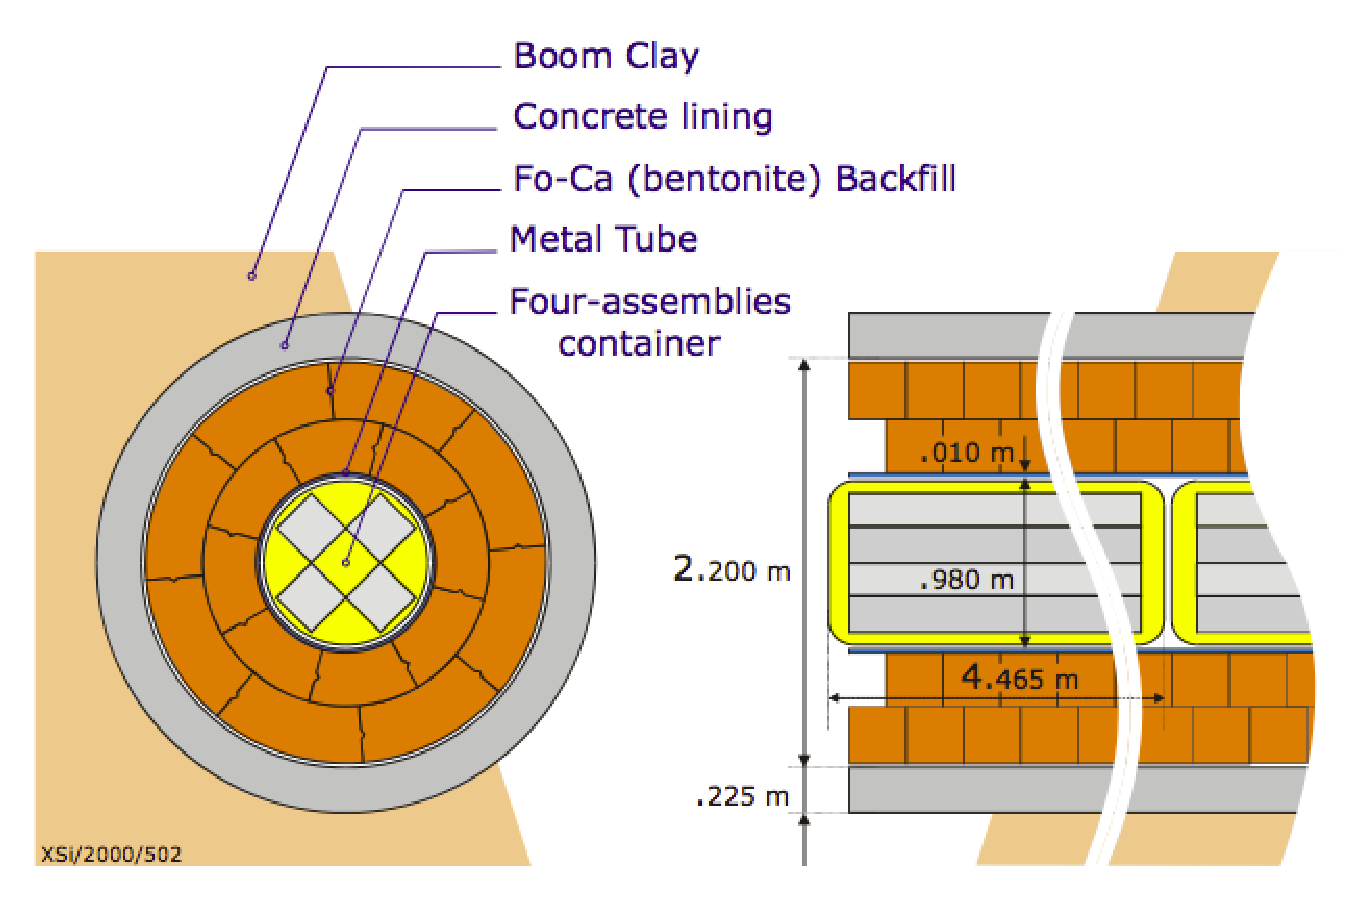
\includegraphics[height=.7\textheight]{./images/belgianClayRedImp.eps}
    \end{center}
    \caption{Belgian reference concept in Boom Clay 
    \cite{von_lensa_red-impact_2008}.}
    \label{fig:belgianClayRedImp}
  \end{figure}

}
\end{frame}

\begin{frame}
  \frametitle{Granite Disposal Environments}
  \footnotesize{

  \begin{figure}[h!]
    \begin{center}
      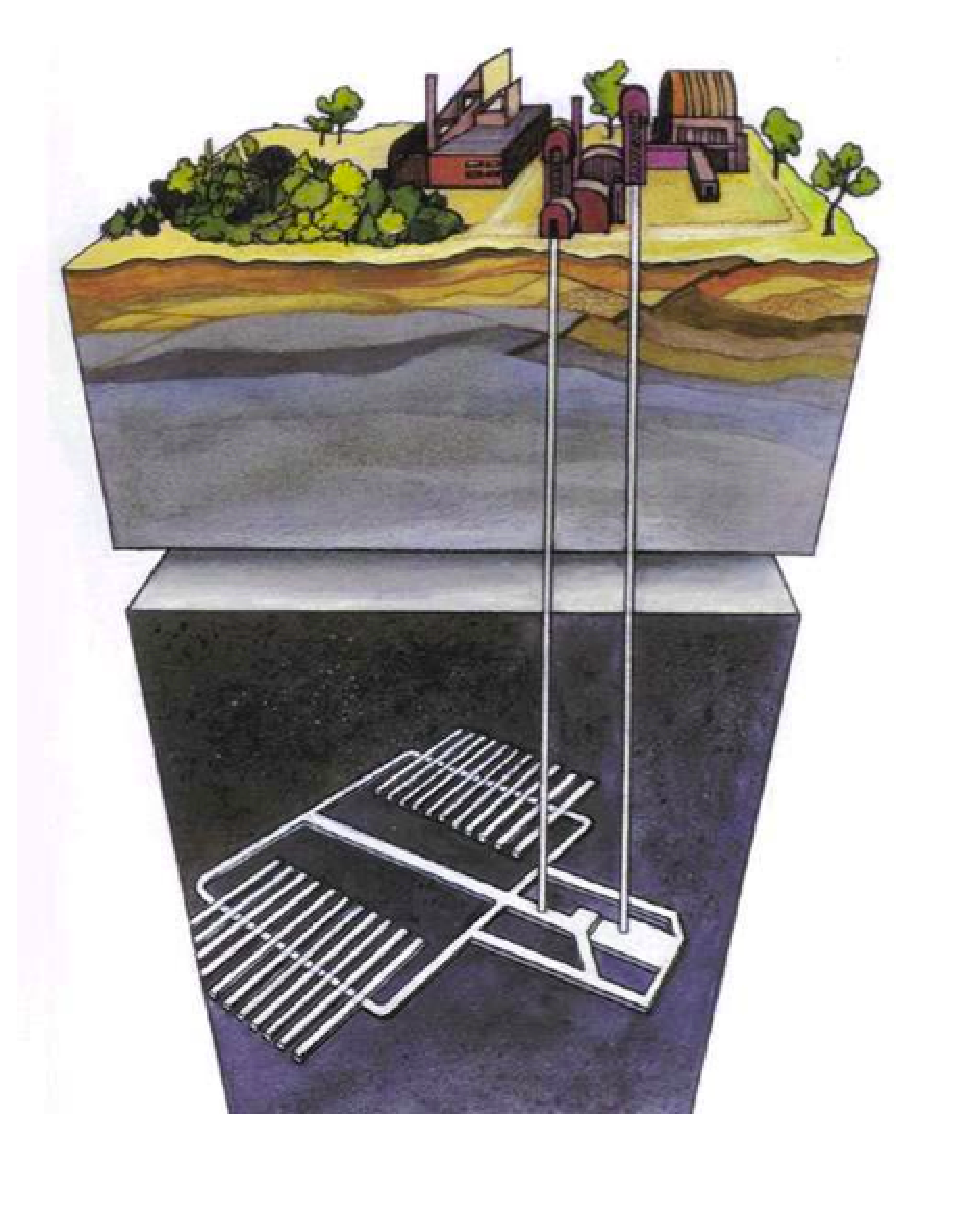
\includegraphics[height=.7\textheight]{./images/czechGraniteRedImp.eps}
    \end{center}
    \caption{Czech reference concept in Granite 
    \cite{von_lensa_red-impact_2008}.}
    \label{fig:czechGraniteRedImp}
  \end{figure}
}
\end{frame}

\begin{frame}
  \frametitle{Salt Disposal Environments}
  \footnotesize{

  \begin{figure}[h!]
    \begin{center}
      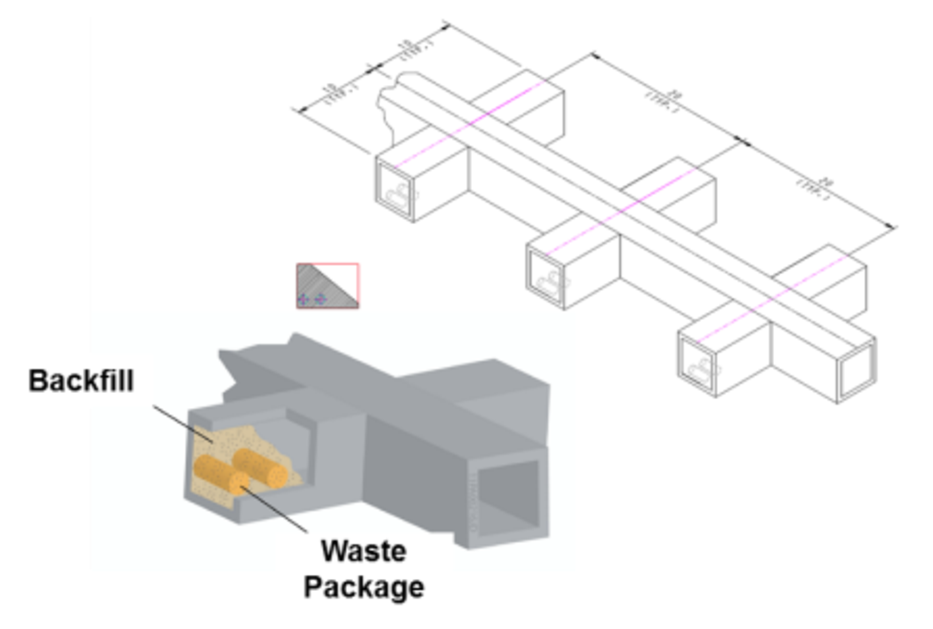
\includegraphics[height=.7\textheight]{./images/carter_salt_layout.eps}
    \end{center}
    \caption{DOE-NE Used Fuel Disposition Campaign  concept in 
    Salt \cite{hardin_generic_2011}.}
    \label{fig:salt_layout}
  \end{figure}
}
\end{frame}
\begin{frame}
  \frametitle{Salt Disposal Environments}
  \footnotesize{

  \begin{figure}[h!]
    \begin{center}
      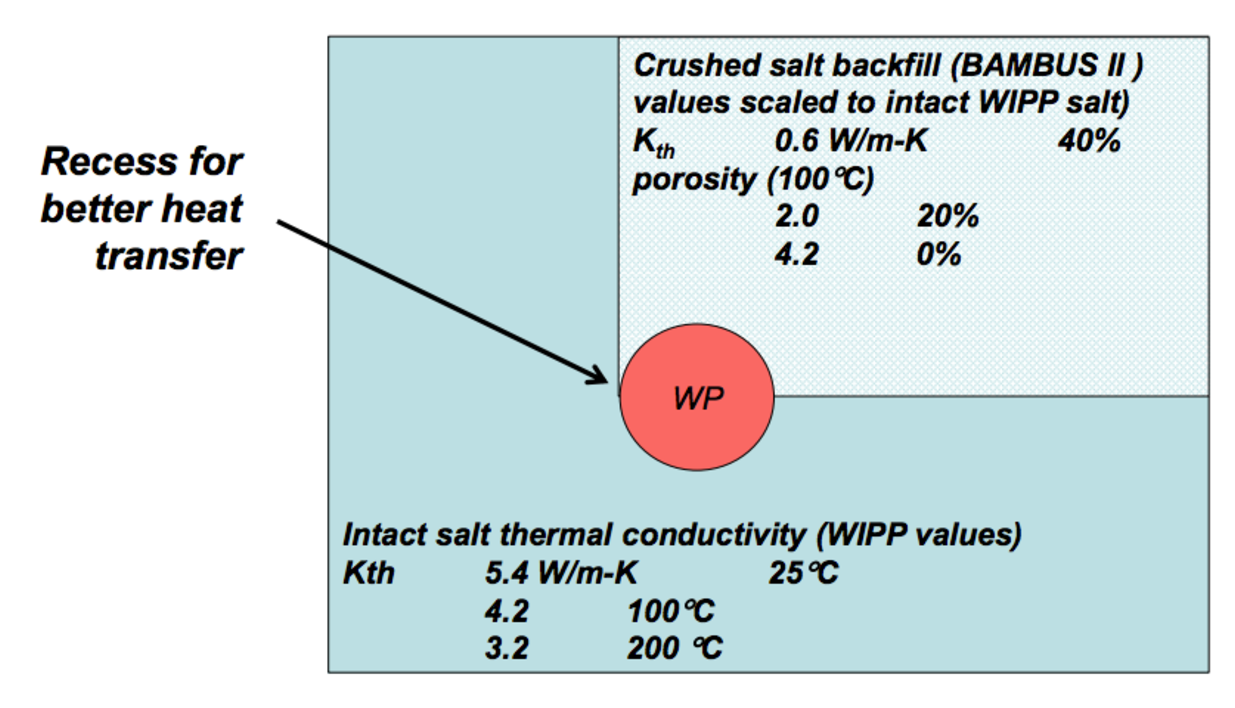
\includegraphics[height=.7\textheight]{./images/hardin_salt_layout.eps}
    \end{center}
    \caption{DOE-NE Used Fuel Disposition Campaign  concept in 
    Salt \cite{hardin_generic_2011}.}
    \label{fig:hardin_salt_layout}
  \end{figure}
}
\end{frame}

\begin{frame}
  \frametitle{Deep Borehole Disposal Environment}
  \footnotesize{

  \begin{figure}[h!]
    \begin{center}
      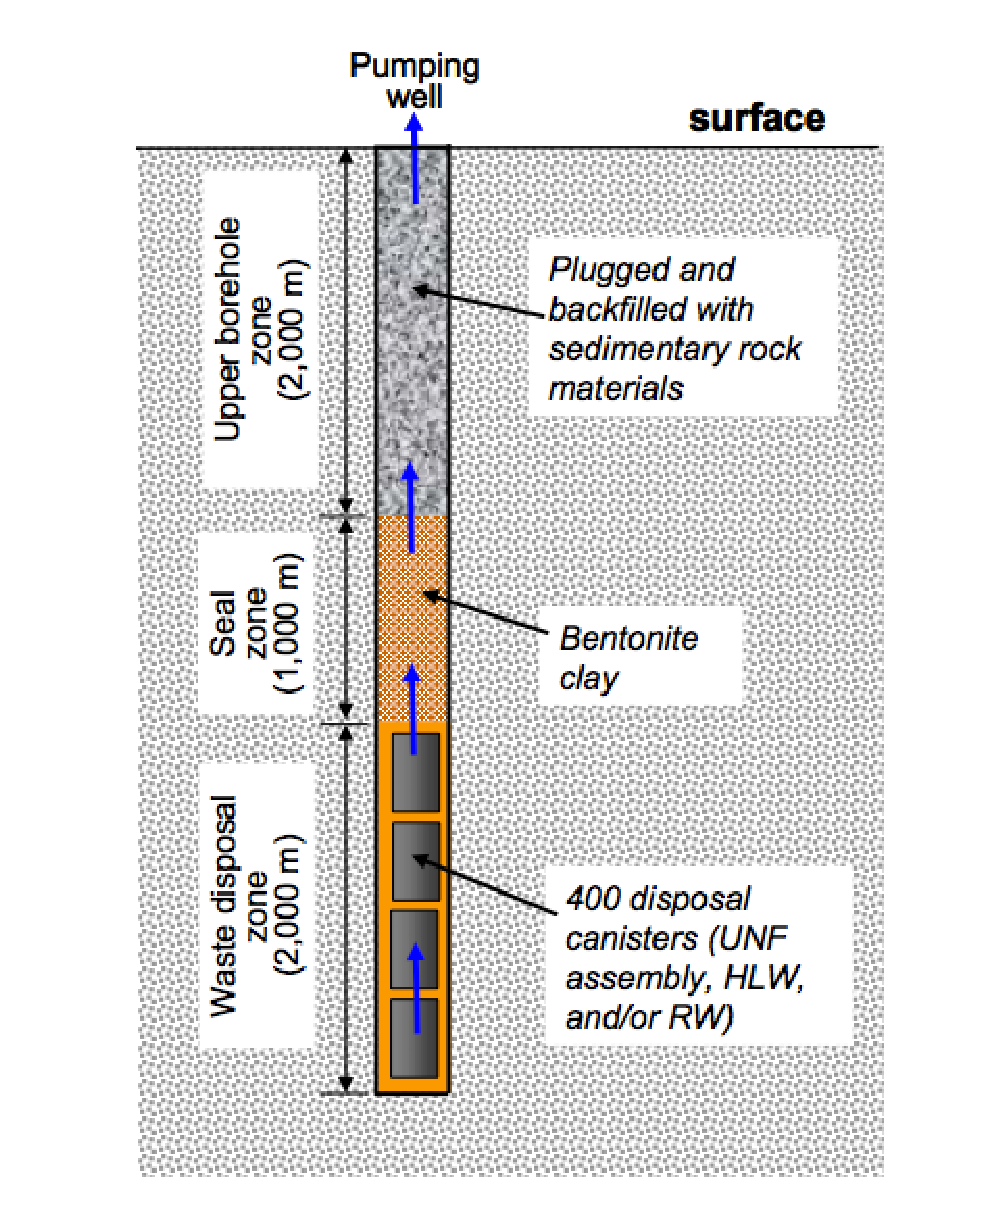
\includegraphics[height=.7\textheight]{./images/boreholeGPAM.eps}
    \end{center}
    \caption{DOE-NE Used Fuel Disposition Campaign Deep Borehole concept 
    \cite{hardin_generic_2011}.}
    \label{fig:boreholeGPAM}
  \end{figure}
}
\end{frame}




\section{International Progress}
\subsection{International Discussion}
\subsection{Finland}
%%--------------------------------%%
\begin{frame}[c]
\frametitle{Finland: Posvia}

\begin{itemize}
\item[\textbf{2001}]  Parliament ratified decision-in-principle siting Olkiluoto, Eurajoki
\item[\textbf{2012}] Construction licence application submitted
\item[\textbf{2015}] Construction licence granted.
\item[\textbf{2020}] Operation licence application to be submitted.
\item[\textbf{2020+}] Final disposal begins.
\end{itemize}
\end{frame}

%%--------------------------------%%
\begin{frame}[c]
\frametitle{Finland: Posiva}
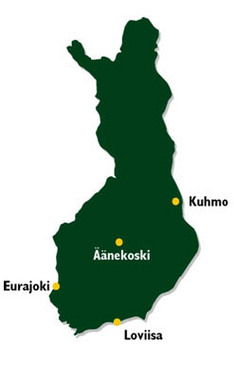
\includegraphics[height=\textheight]{./images/finland-site}
\cite{posiva_safety_2017}
\end{frame}


%%--------------------------------%%
\begin{frame}[c]
\frametitle{Finland: Posvia: KBS-3V Concept}
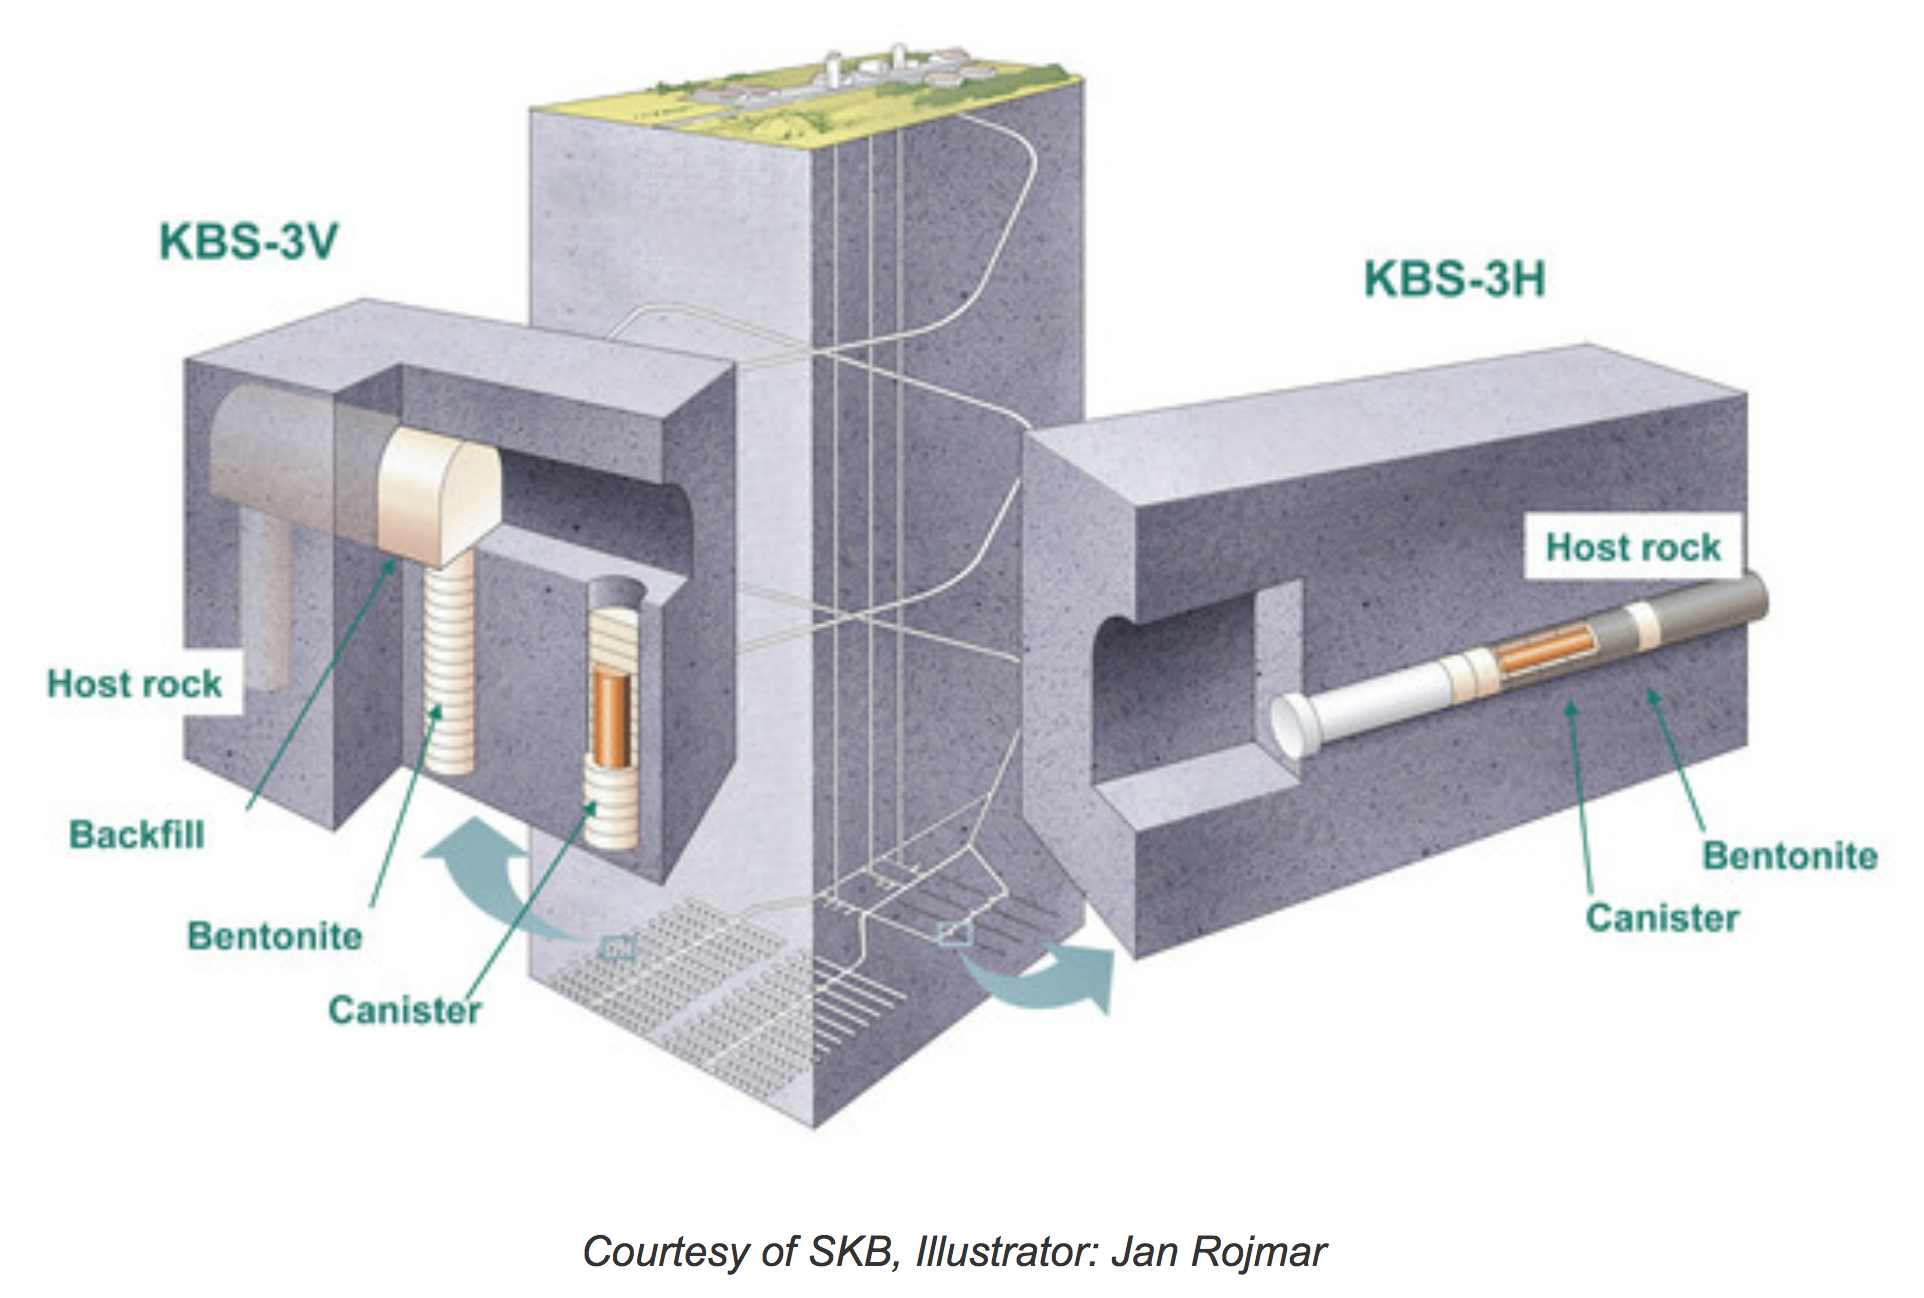
\includegraphics[width=\textwidth]{./images/finland-concept}
\end{frame}
%%--------------------------------%%
\begin{frame}[c]
\frametitle{Sweden: SKB}
\frametitle{Finland: Posvia: KBS-3V Concept}
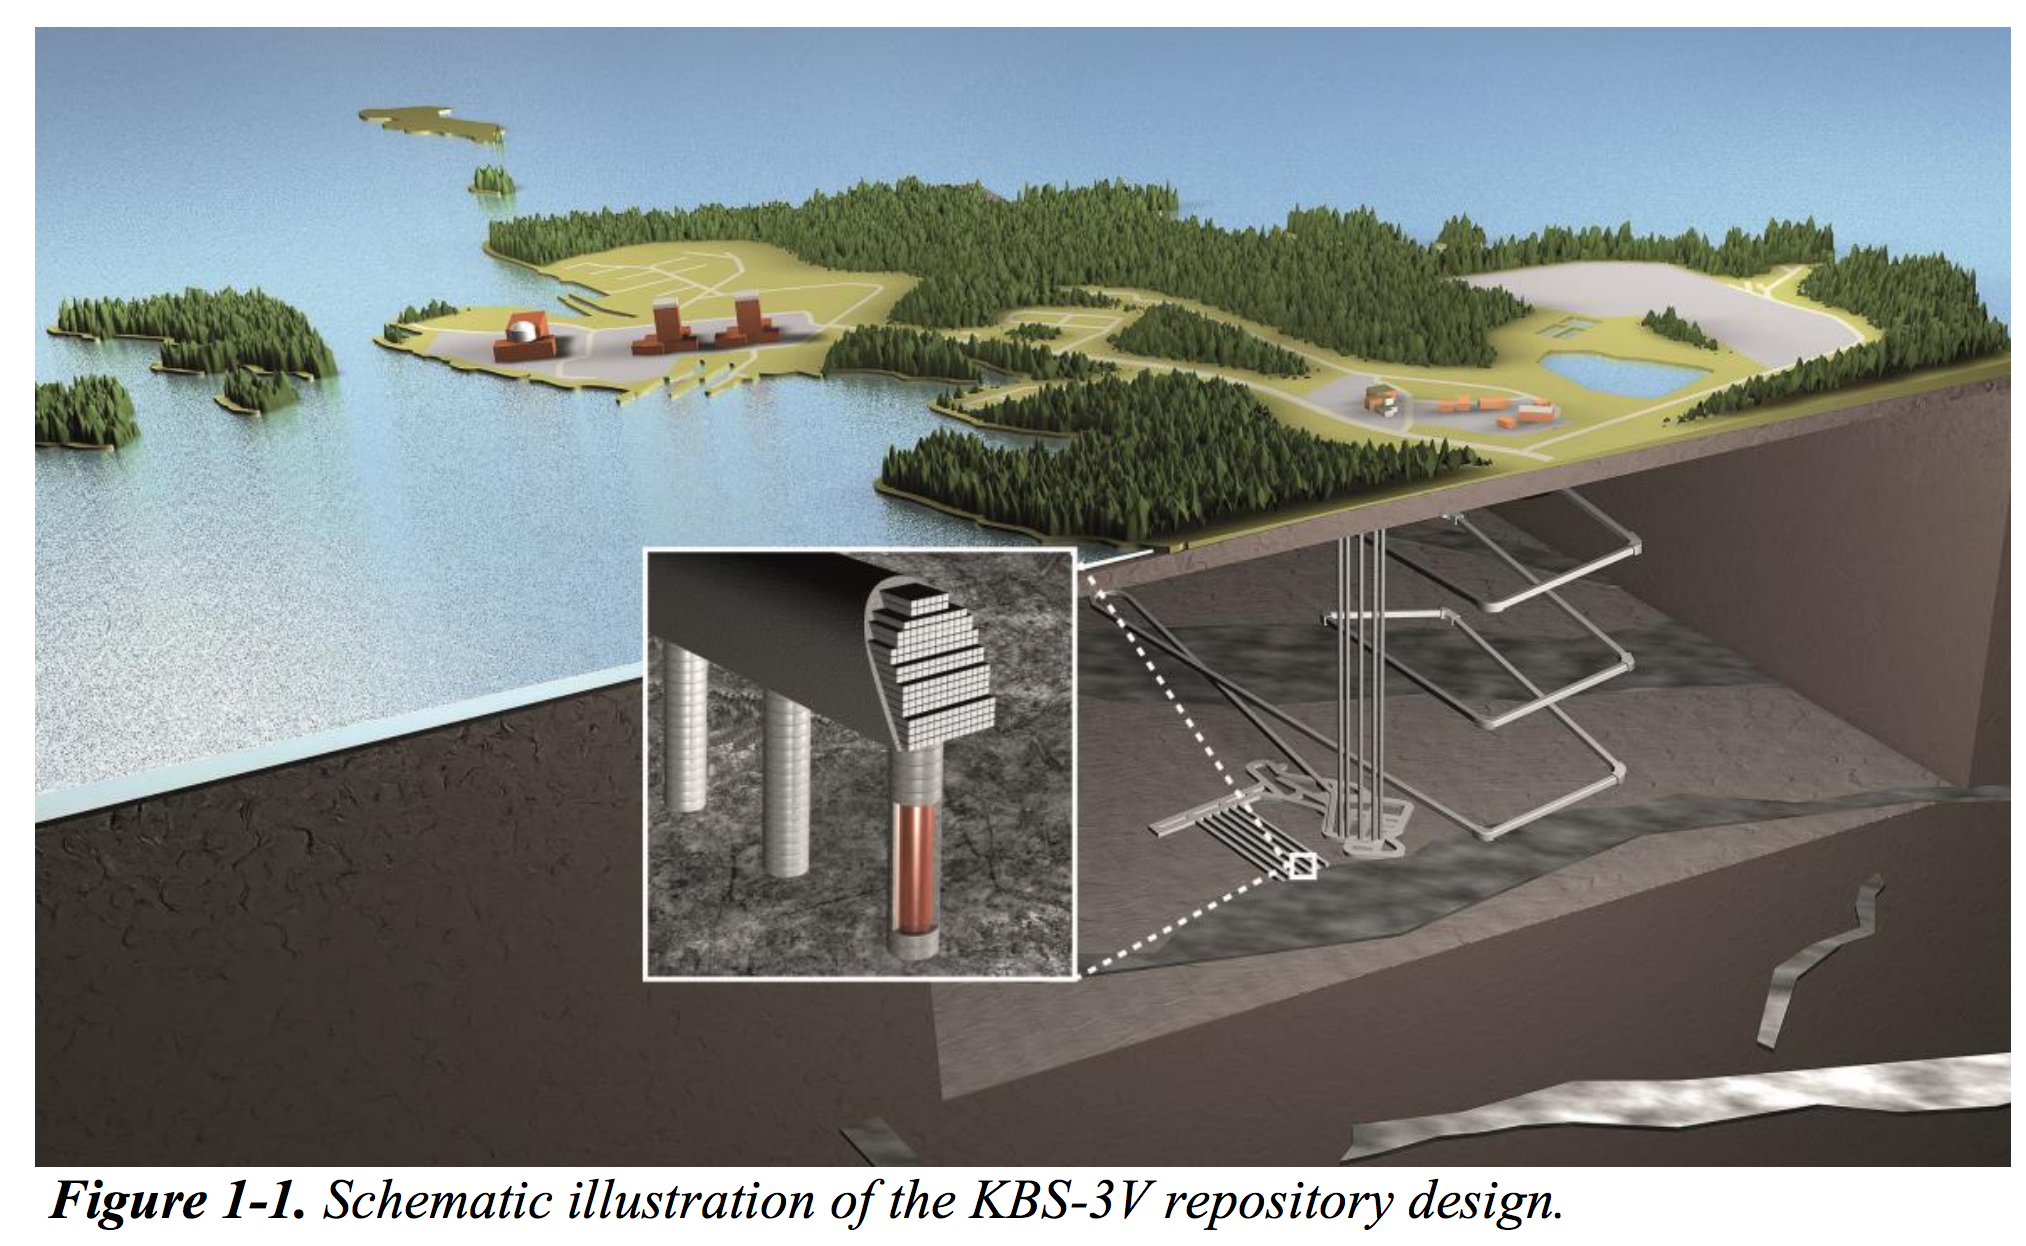
\includegraphics[width=\textwidth]{./images/finland-concept-cartoon}
\end{frame}

\subsection{Sweden}
%%--------------------------------%%
\begin{frame}[c]
\frametitle{Sweden: SKB}

\cite{skb_safety_2017}
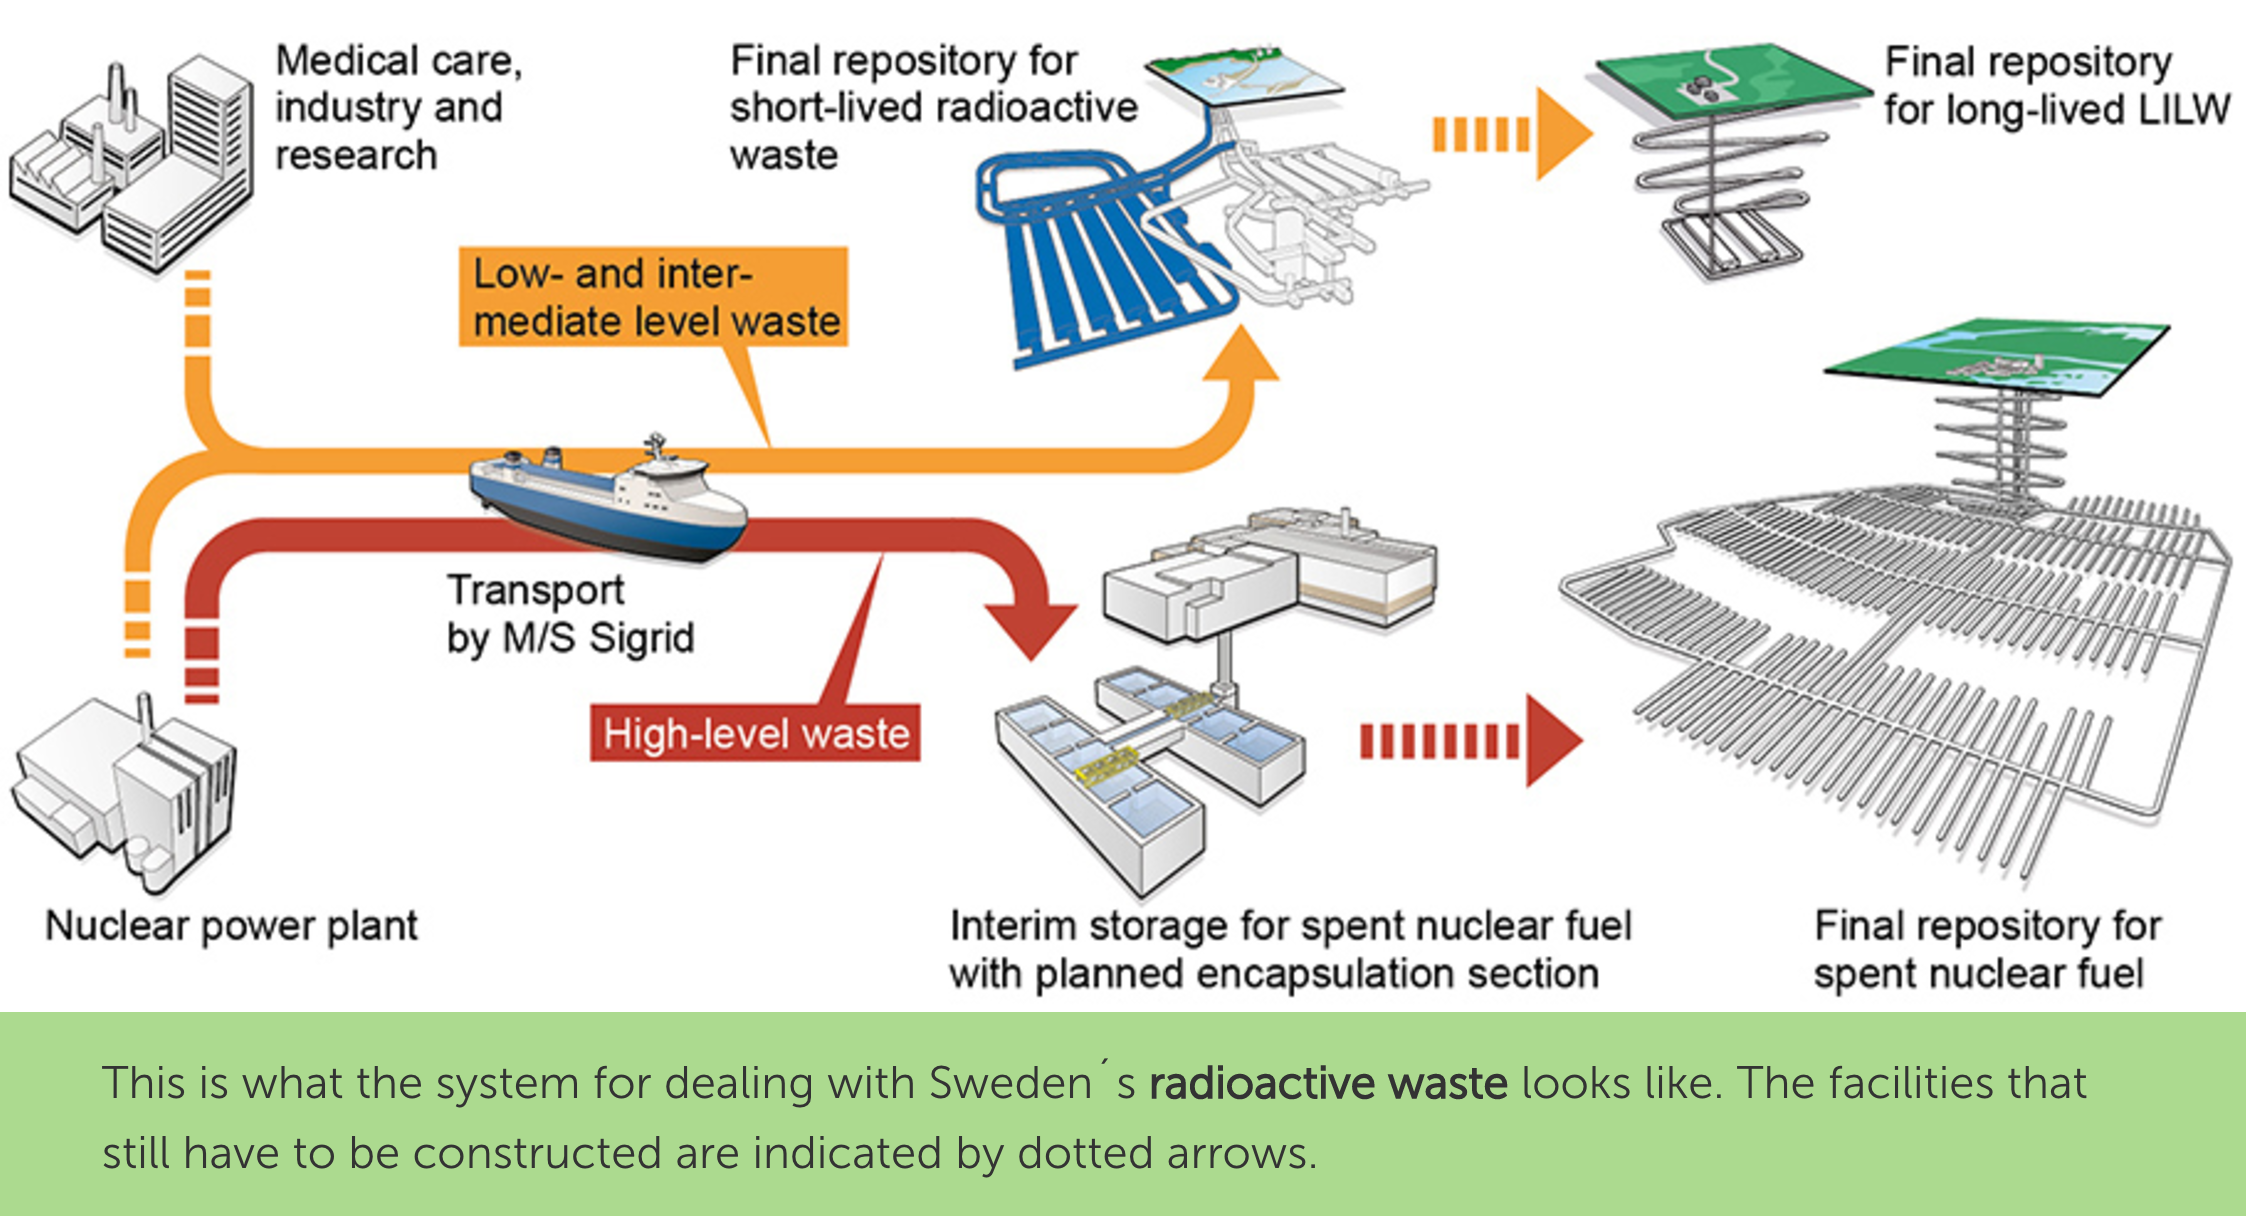
\includegraphics[width=\textwidth]{./images/sweden-plan}
\end{frame}


%%--------------------------------%%
\begin{frame}[c]
\frametitle{Sweden: Site}
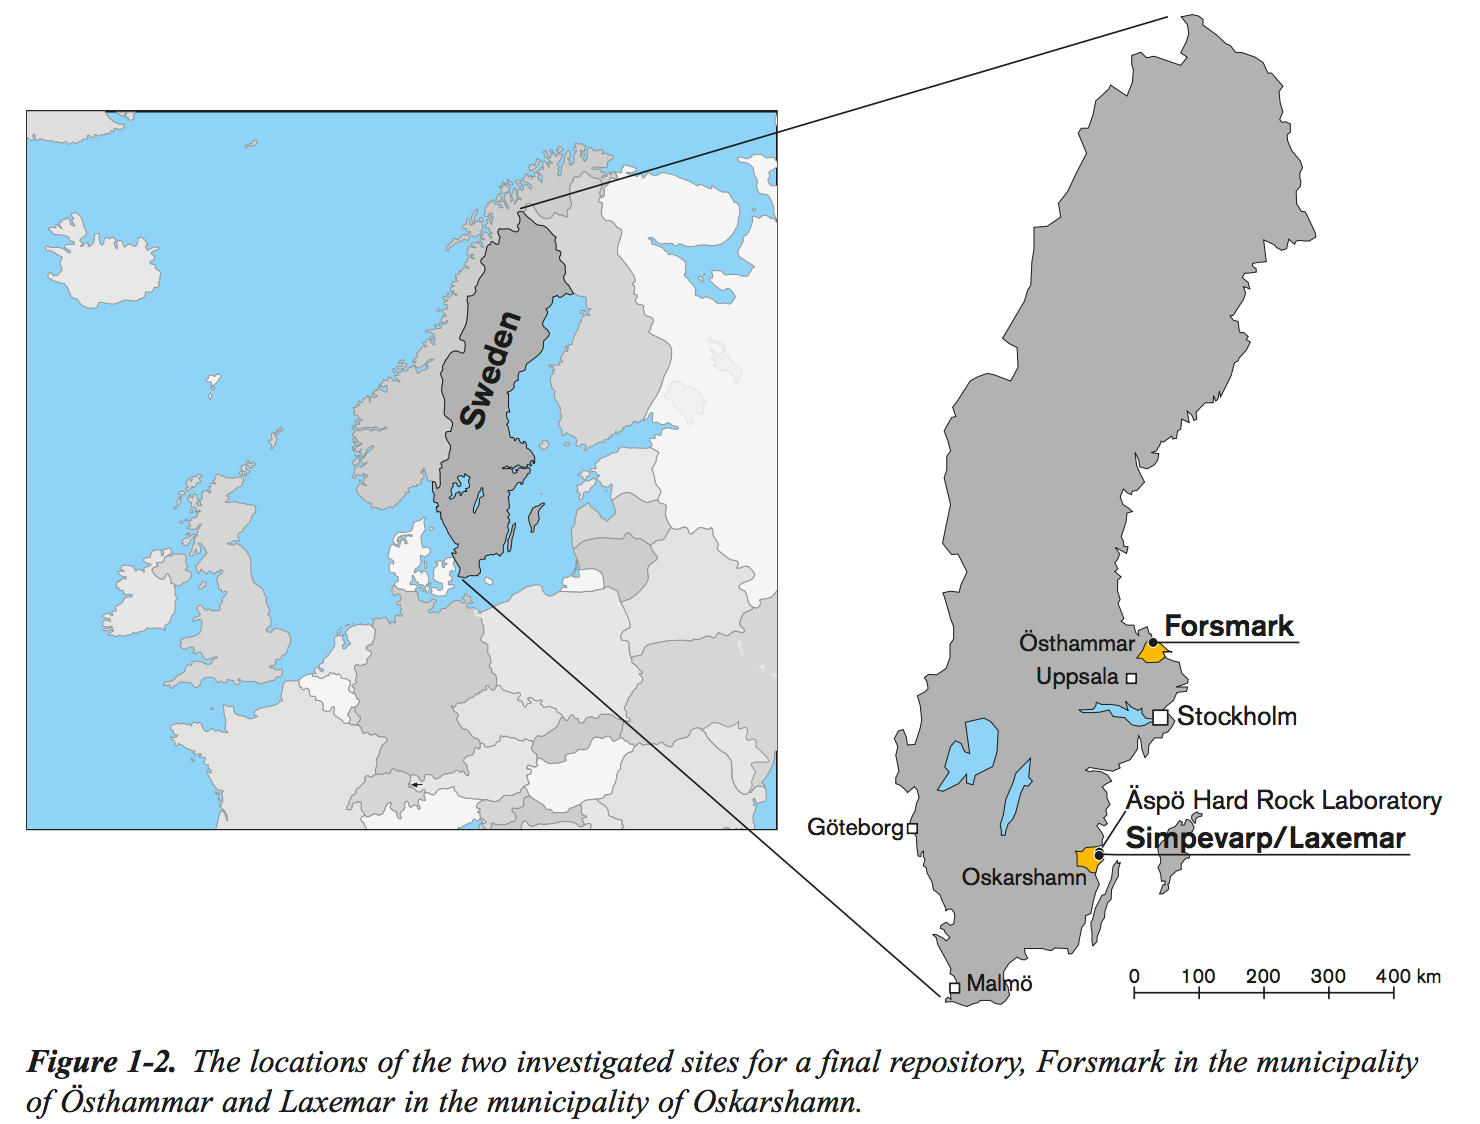
\includegraphics[width=\textwidth]{./images/sweden-site-selection}
\cite{skb_safety_2017}
\end{frame}

%%--------------------------------%%
\begin{frame}[c]
\frametitle{Sweden: Clab}

Clab - the Central Interim Storage Facility for Spent Nuclear Fuel is located at Simpevarp about 25 kilometres north of Oskarshamn. This is where all the spent nuclear fuel from Swedish nuclear power plants is kept while waiting for the final repository to begin operating.

\end{frame}


%%--------------------------------%%
%%--------------------------------%%
\begin{frame}[c]
\frametitle{Sweden: Short-Lived Radioactive Waste}
SKB’s Final Repository for Short-Lived Radioactive Waste is located
At Forsmark in the municipality of \"{O}sthammar. The facility started operating in 1988 and was then the first of its kind in the world.

\begin{itemize}
\item \textbf{Operational start}: 1988
\item \textbf{Capacity}: Approx. 63,000 cubic metres
\item \textbf{Receiving capacity}: Approx. 600 cubic metres per year
\item \textbf{Operational and maintenance staff}: Approx. 30
\item \textbf{Above ground}: Offices and workshops, terminal building, ventilation plant
\item \textbf{Underground}: Four rock vaults, one silo, control room
\item \textbf{Operating costs}: Approx. SEK 40 million per year
\end{itemize}

The SFR is situated 50 metres below the bottom of the Baltic and comprises four 160-metre long rock vaults and a chamber in the bedrock with a 50-metre high concrete silo for the most radioactive waste. Two parallel kilometre-long access tunnels link the facility to the surface.
\end{frame}
%%--------------------------------%%
\begin{frame}[c]
\frametitle{Sweden: SKB}

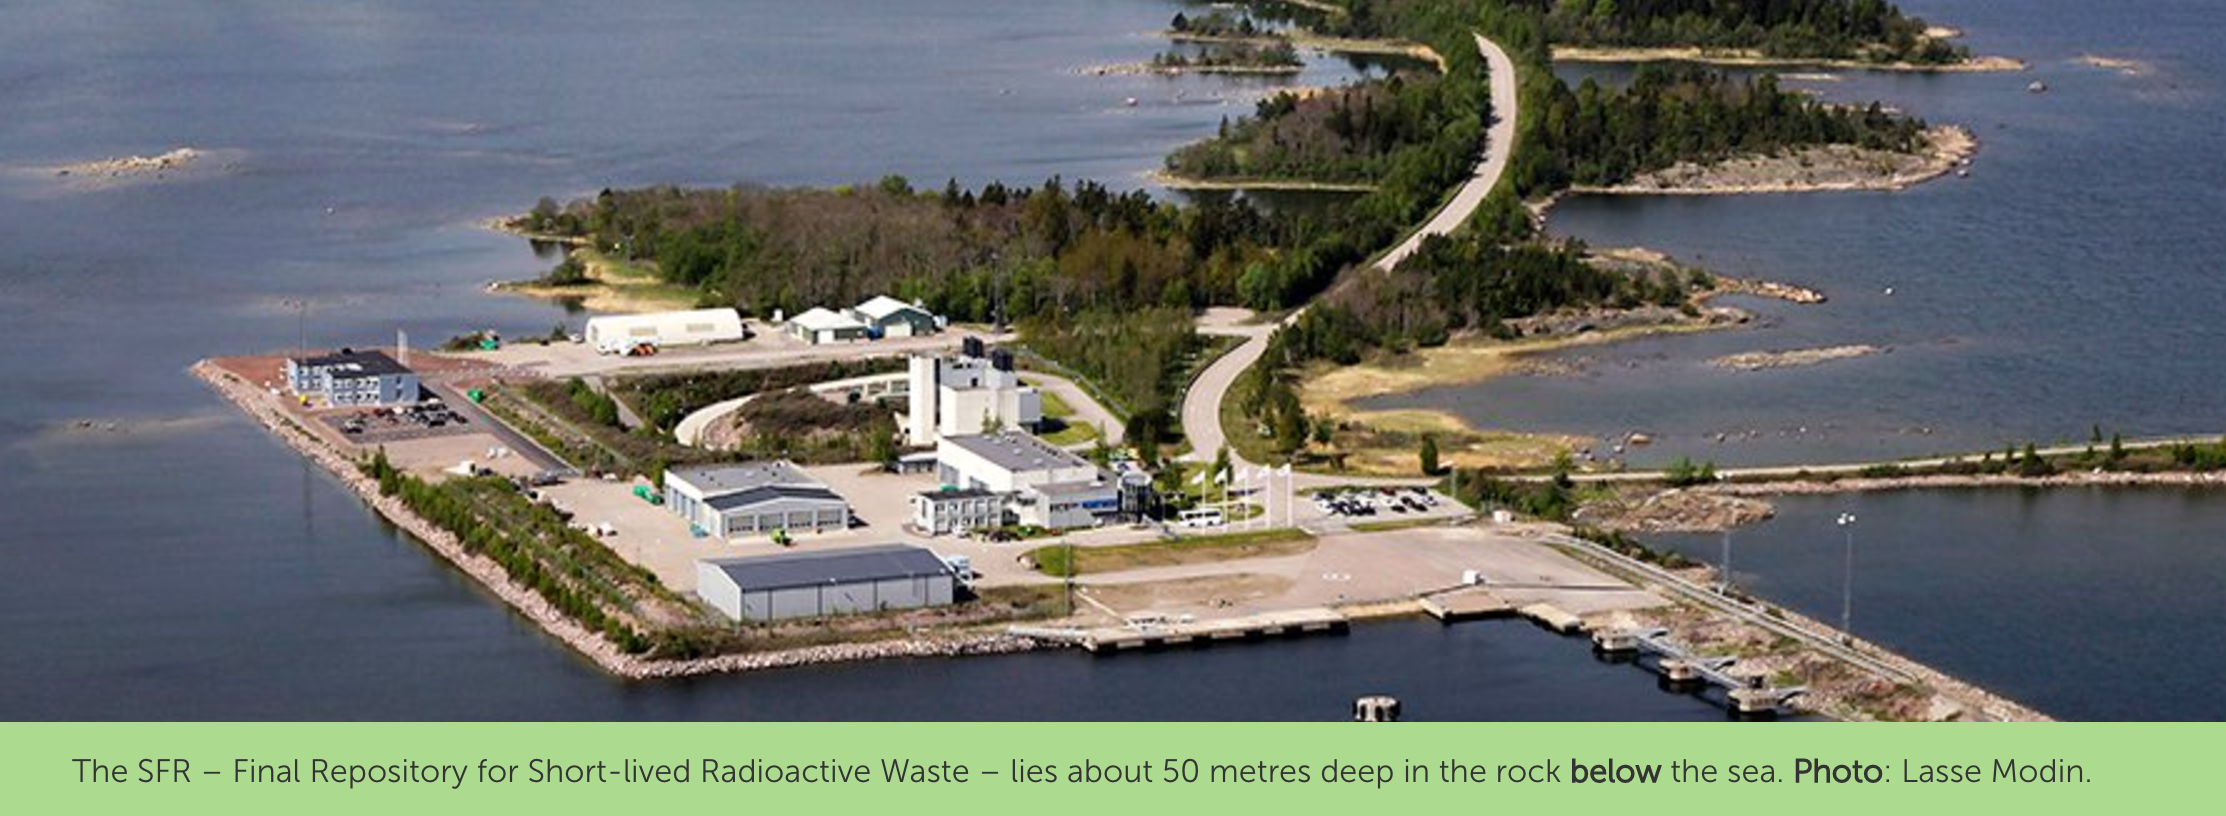
\includegraphics[width=\textwidth]{./images/sweden-sfr}

\end{frame}

%%--------------------------------%%
%%--------------------------------%%
\begin{frame}[c]
\frametitle{Sweden: Final Disposal}

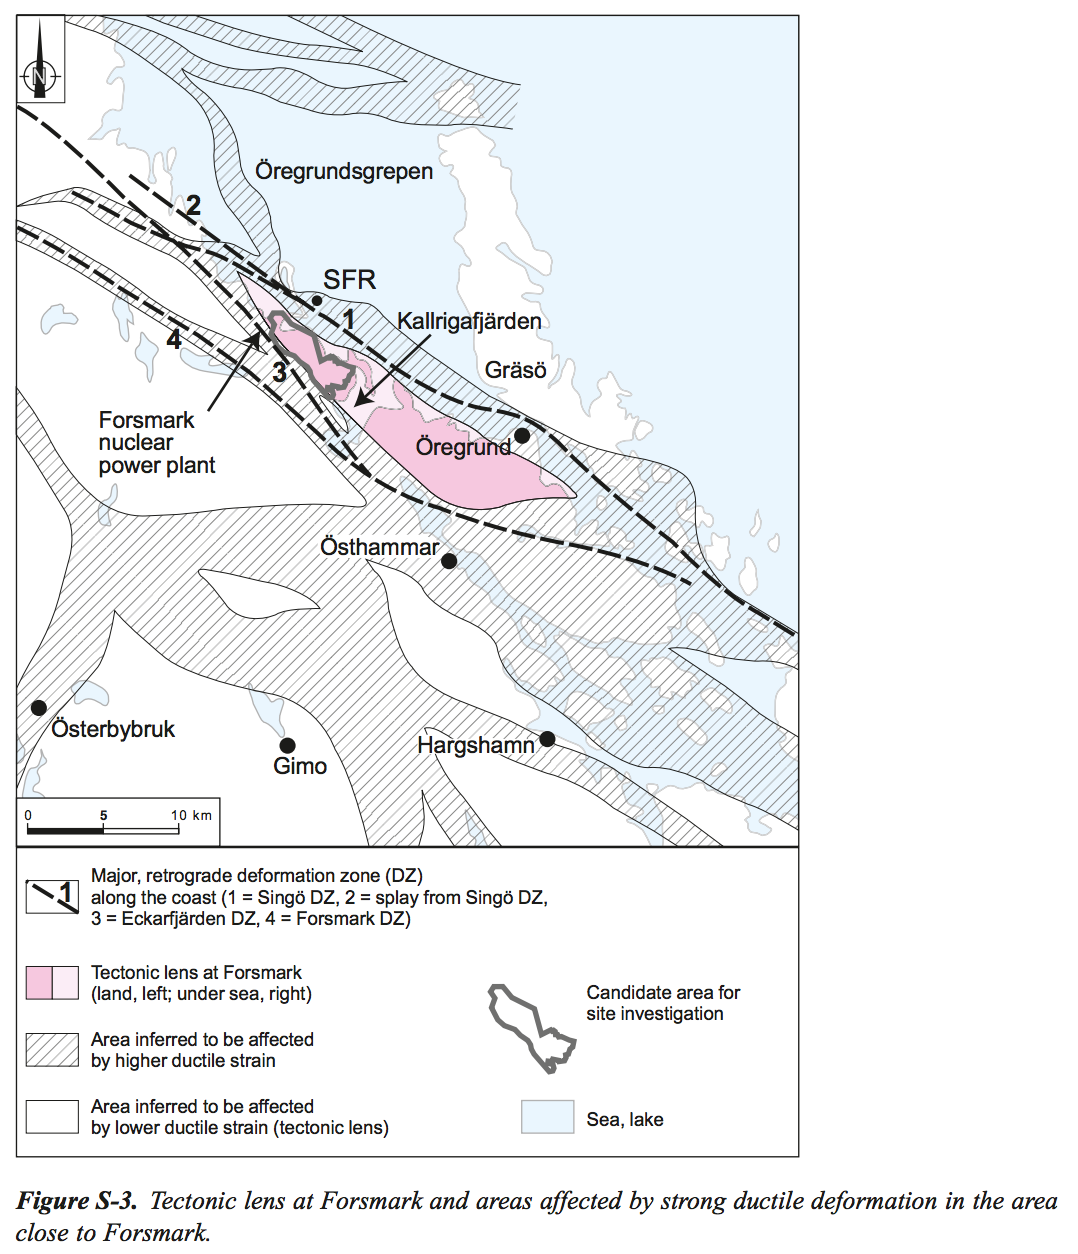
\includegraphics[height=\textheight]{./images/sweden-forsmark-map}
From \cite{skb_long-term_2011}

\end{frame}
%%--------------------------------%%
\begin{frame}[c]
\frametitle{Sweden: Final Disposal}
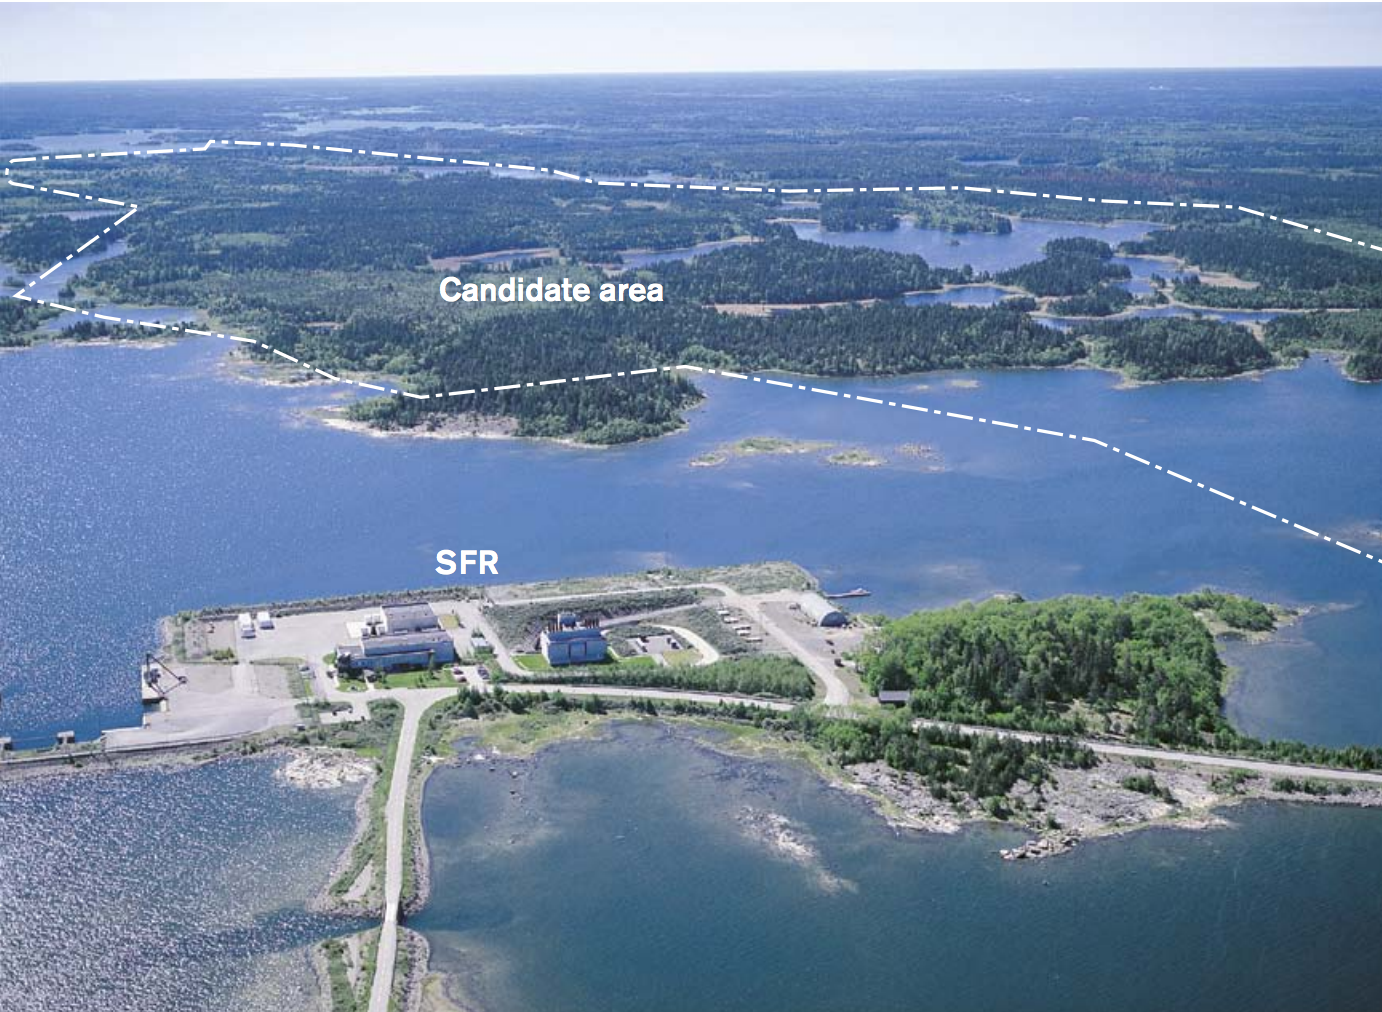
\includegraphics[height=\textheight]{./images/sweden-forsmark-candidate}
From \cite{skb_long-term_2011}
\end{frame}

%%--------------------------------%%
\begin{frame}[c]
\frametitle{Sweden: Final Disposal}
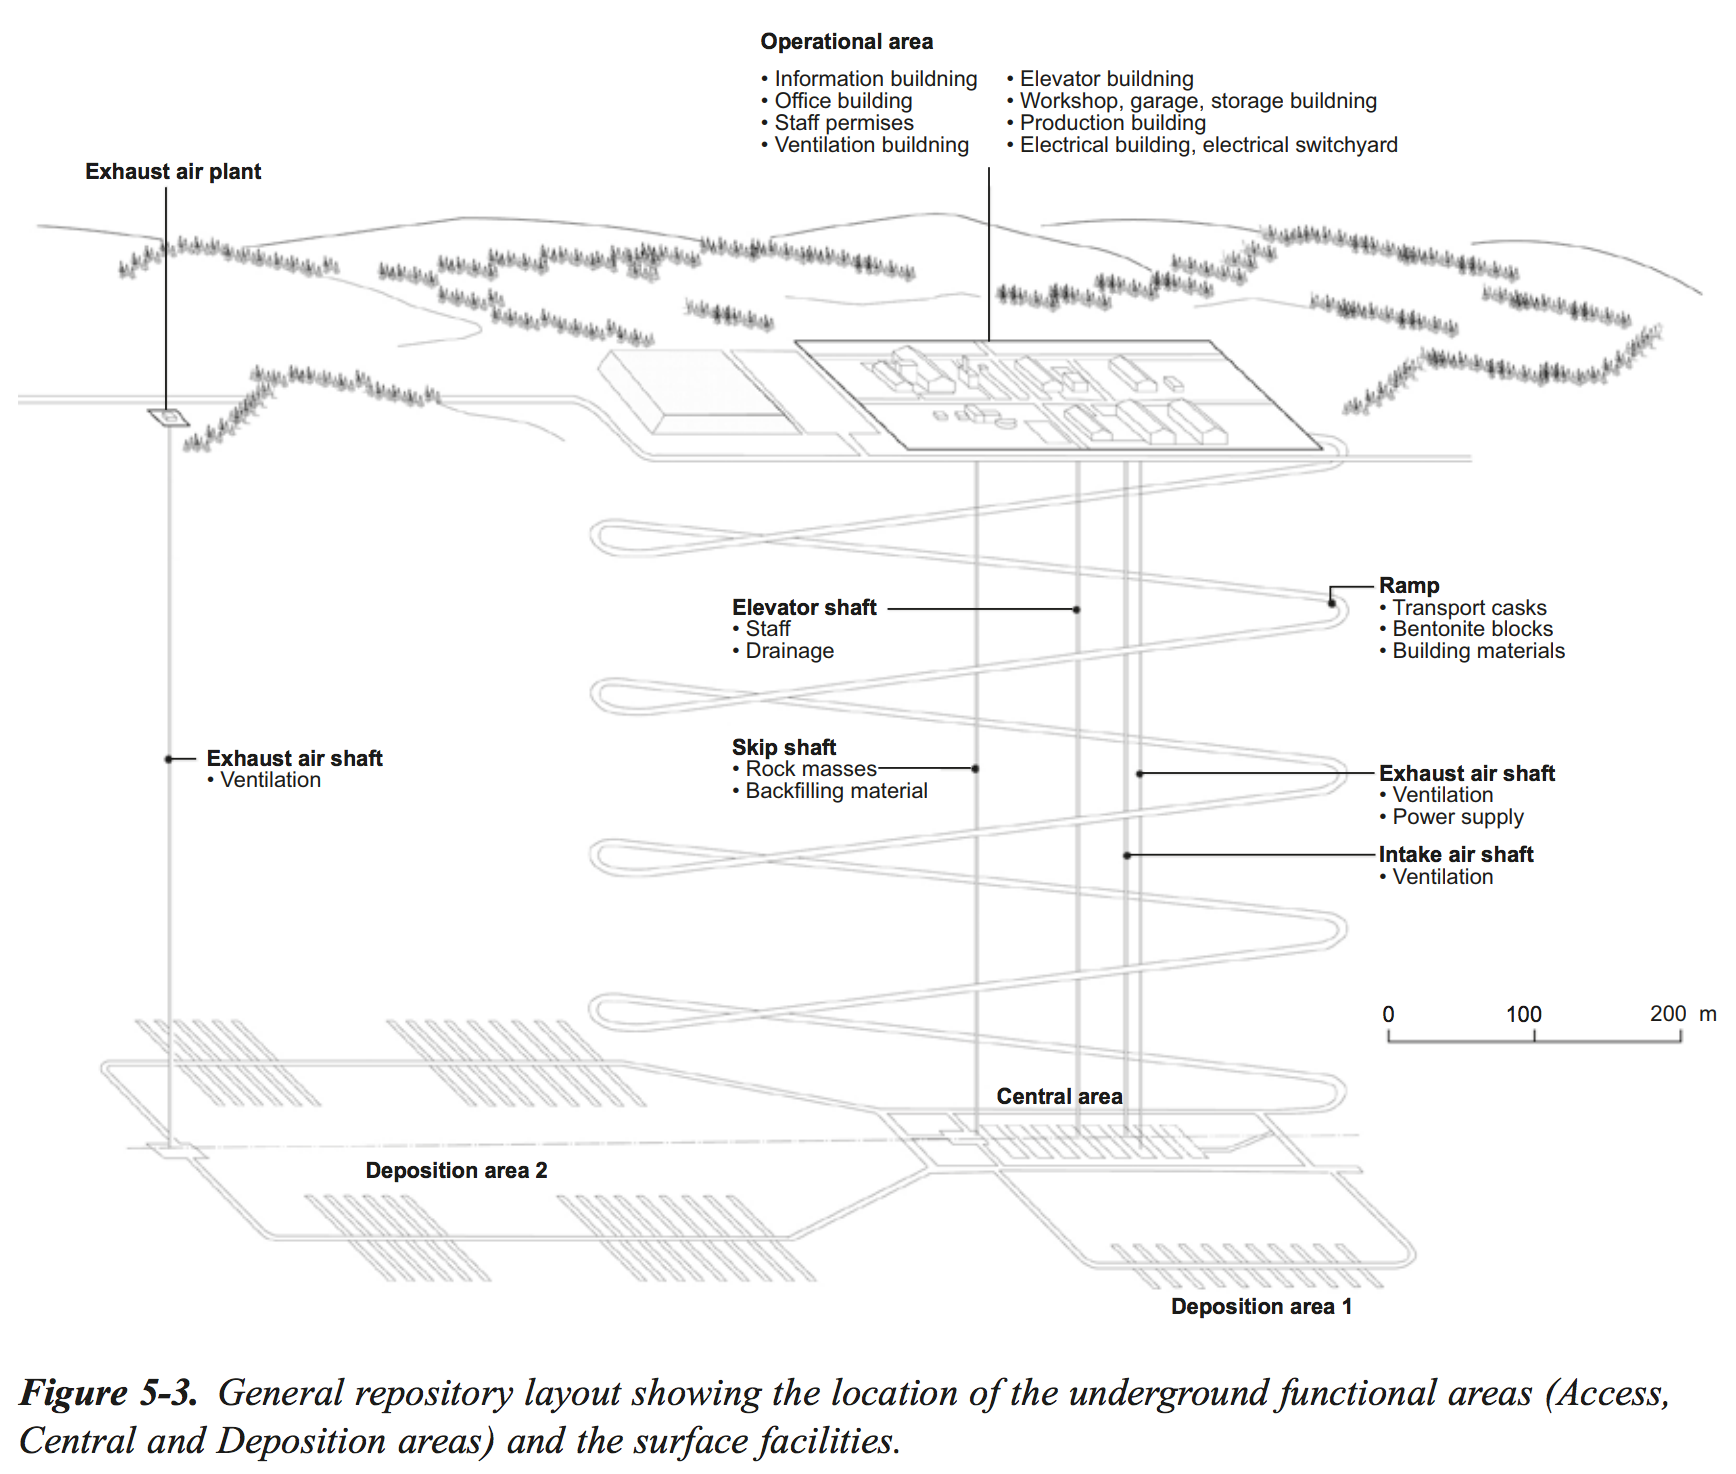
\includegraphics[height=\textheight]{./images/sweden-forsmark-design}
From \cite{skb_long-term_2011}
\end{frame}

%%--------------------------------%%
\begin{frame}[c]
\frametitle{Sweden: Final Disposal}
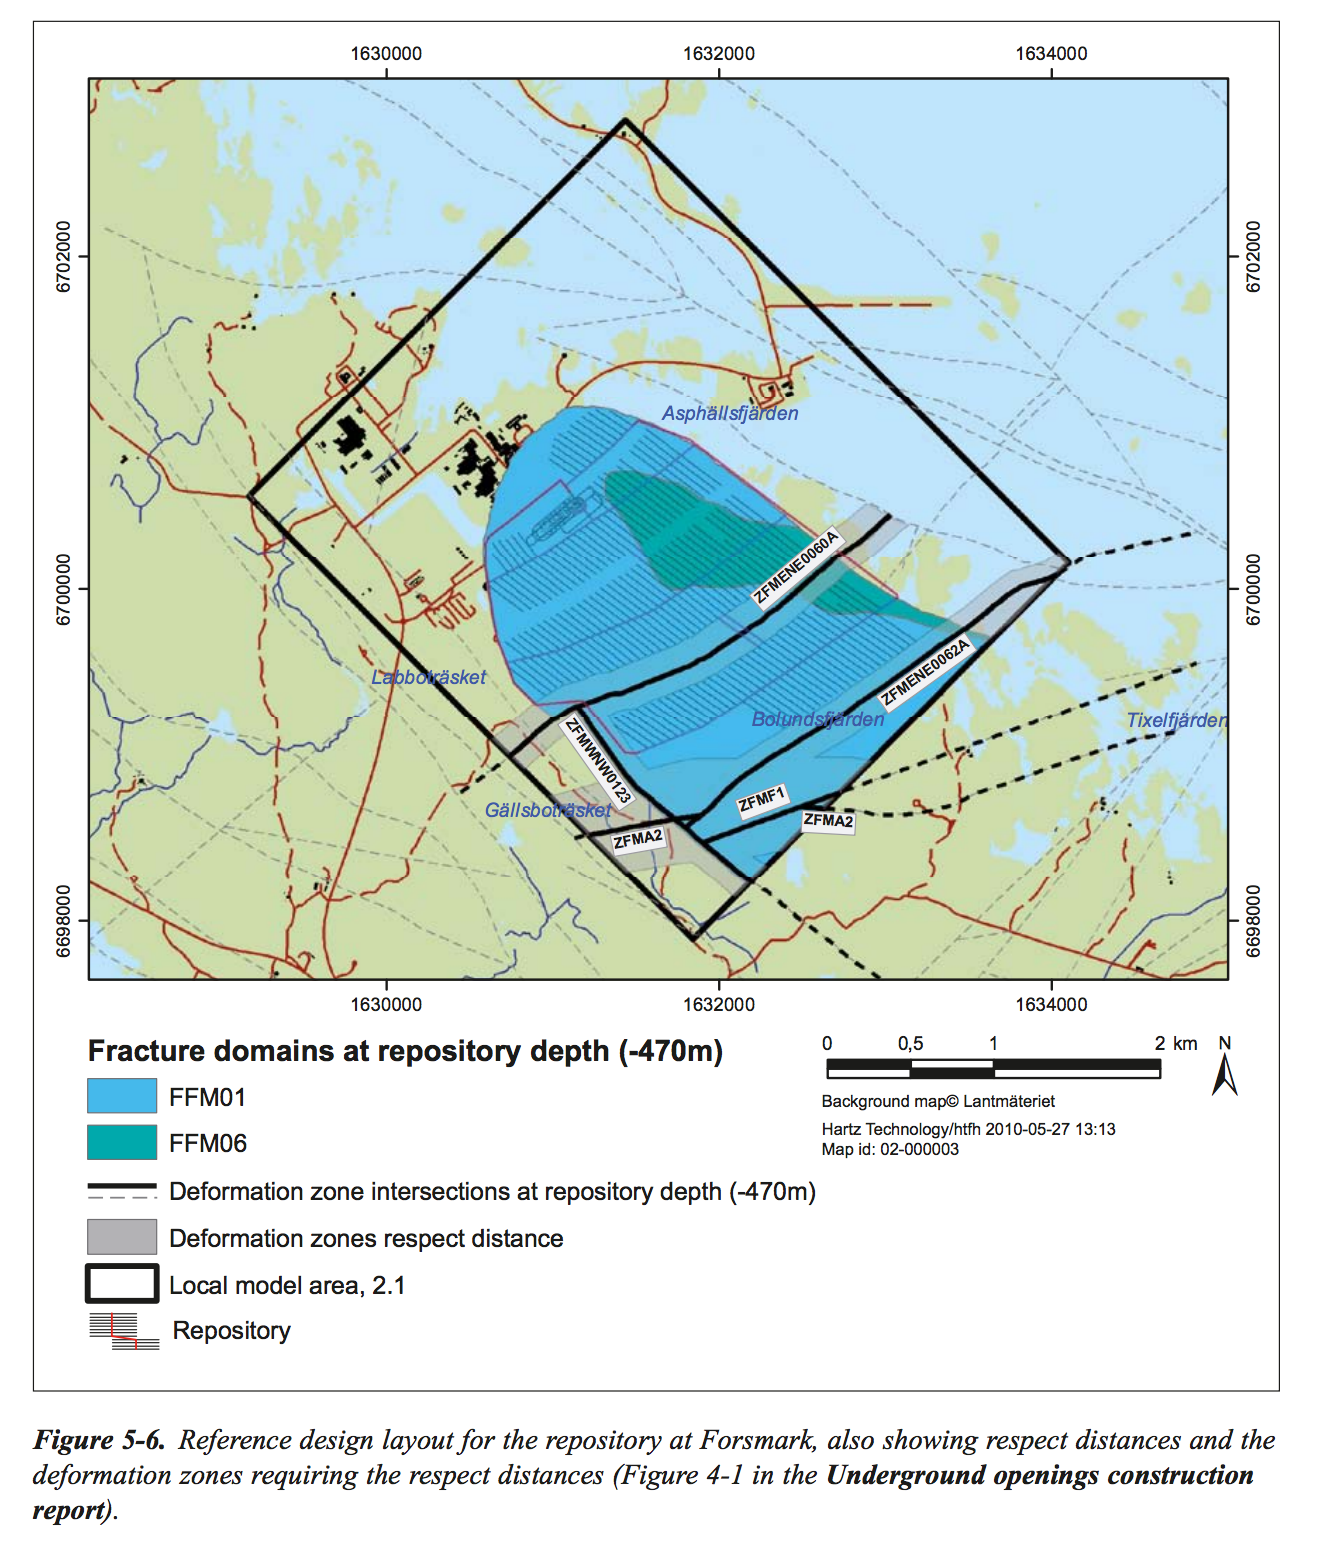
\includegraphics[height=\textheight]{./images/sweden-forsmark-fractures}
From \cite{skb_long-term_2011}
\end{frame}


%%--------------------------------%%
\begin{frame}[c]
\frametitle{Sweden: Transport By Sea}

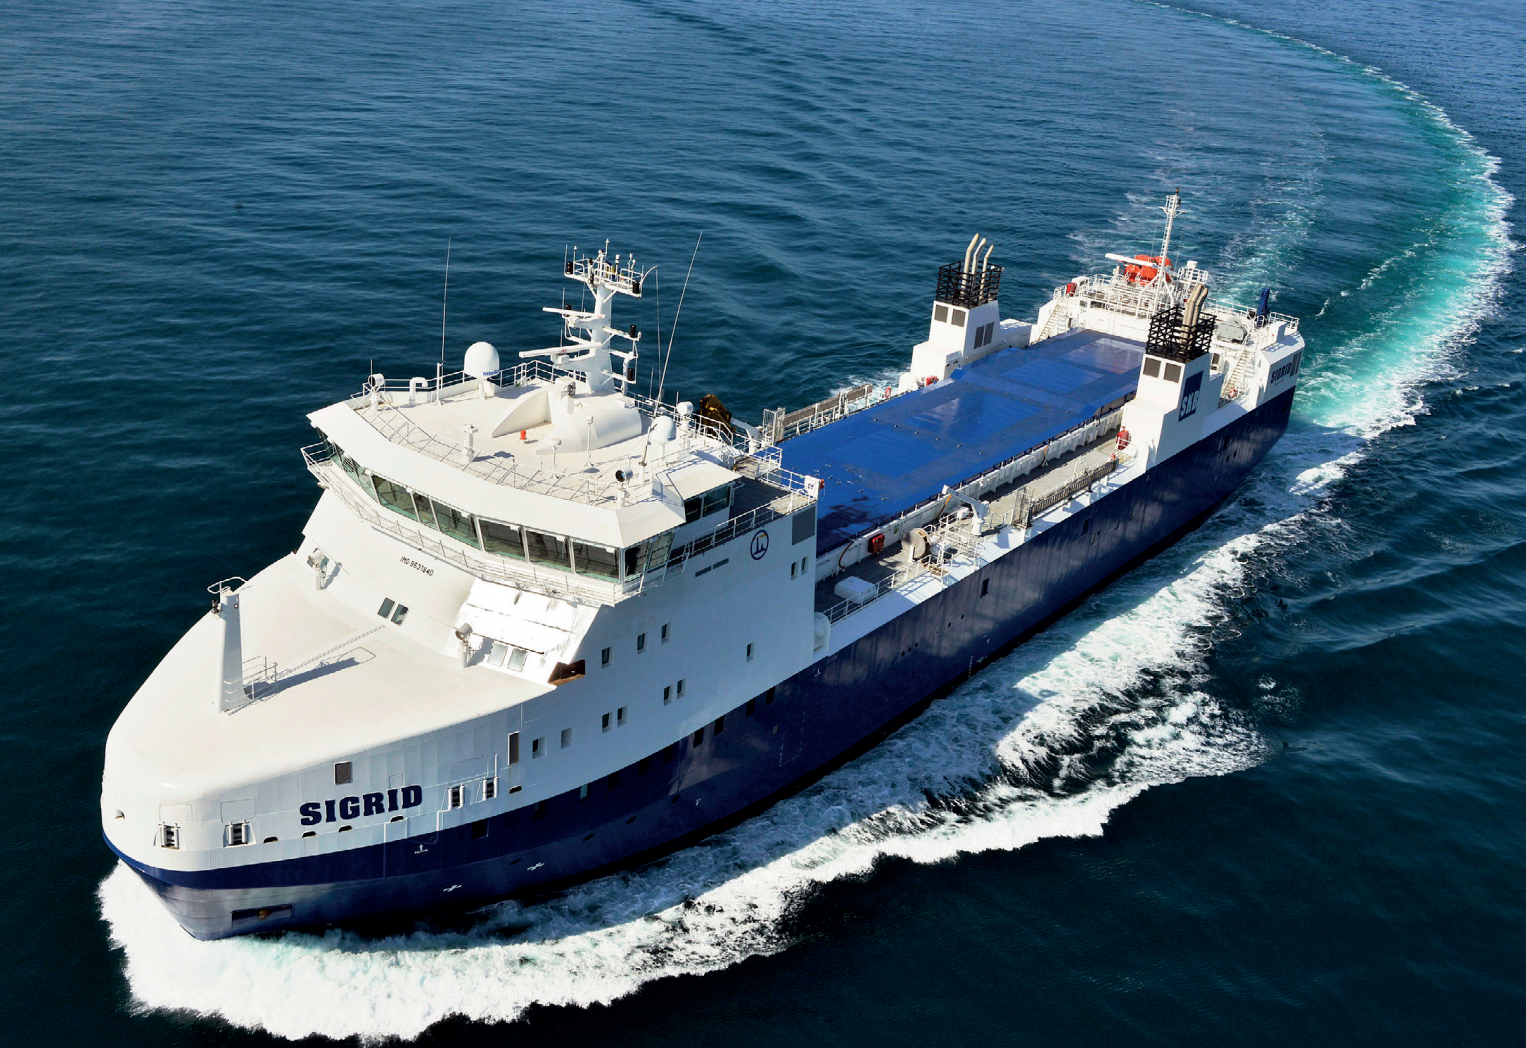
\includegraphics[height=0.9\textheight]{./images/sweden-sigrid}


Sigrid, the vessel which replaced Sigyn in 2013.

\end{frame}

%%--------------------------------%%
\begin{frame}[c]
\frametitle{Sweden: Transport By Sea}
\begin{center}
\begin{itemize}
\item[\textbf{Length overall}] 99.5 metres
                \item \textbf{Primary cargo}: Radioactive waste and spent nuclear fuel
                \item \textbf{Cargo capacity}: 12 transport casks or 40 freight containers
                \item \textbf{Draught}: 4.5 metres
                \item \textbf{Deadweight tonnage}: 1,600 tonnes
        \end{itemize}
\end{center}
\end{frame}

\section{Challenges}
\subsection{Challenge: Financial}
\include{cost}
\subsection{Challenge: Political}
\include{political}
\subsection{Challenge: Security}
\include{security}
\subsection{Challenge: Geological}
\subsubsection{Metrics}

%%----------------------------------------%%
\begin{frame}
  \frametitle{Performance Metrics}
  \begin{itemize}
  \item Dose
  \item Environmental Release 
  \item Repository Footprint
  \item Cost
  \item ...
\end{itemize}
\end{frame}

\subsubsection{Thermal Loading}

%%----------------------------------------%%
\begin{frame}
  \frametitle{Thermal Capacity in Various Geologies}
\footnotesize{
  \begin{figure}[htbp!]
  \begin{center}
    \includegraphics[width=0.7\textwidth]{./images/greenberg_thermal.eps}
  \end{center}
  \caption{The varying thermal limits, thermal conductivities, and thermal 
    diffusivities of various geologies result in differing heat capacities to 
    similar waste \cite{greenberg_application_2012}.}
  \label{fig:greenberg_thermal}
\end{figure}

}
\end{frame}

\subsubsection{Radionuclide Transport and Release}

%%----------------------------------------%%
\begin{frame}
  \frametitle{Release Mechanisms}
  \begin{itemize} 
  \item Human Disruption
  \item Natural Disruption
  \item Barrier Dissolution
  \item Advection
  \item Diffusion
  \item Sorption
  \item Solubility Limitation
  \item ... 
  \end{itemize}
\end{frame}

%%----------------------------------------%%
\begin{frame}
\frametitle{Solubility Sensitivity In A Clay Model}
\begin{figure}[ht]
  \centering
  \includegraphics[width=0.7\linewidth]{./images/Solubility_Summary.eps}
  \caption{Solubility limit sensitivity. The peak annual dose due to an 
  inventory, $N$, of each isotope.}
  \label{fig:SolSum}
\end{figure}
\end{frame}

%%----------------------------------------%%
\begin{frame}
\frametitle{Retardation Sensitivity In A Clay Model}
\begin{figure}[ht]
  \centering
  \includegraphics[width=0.7\linewidth]{./images/Partitioning_Summary.eps}
  \caption{$K_d$ sensitivity.  The peak annual dose due to an inventory, 
  $N$, of each isotope.}
  \label{fig:KdSum}
\end{figure}
\end{frame}

%%----------------------------------------%%
\begin{frame}[c]
  \frametitle{Example : Vertical Advective Velocity and Diffusion Coefficient}
\begin{figure}[htp!]
\centering
\includegraphics[width=0.8\textwidth]{./images/Se-79.eps}
\caption{$^{79}Se$.  $Se$ is non sorbing, but solubility limited in clay.  For low vertical advective velocity, the system is diffusion dominated.}
\label{fig:VAdvVelSe79}
\end{figure}
\end{frame}

%%----------------------------------------%%
\begin{frame}[c]
  \frametitle{Example : Vertical Advective Velocity and Diffusion Coefficient}
\begin{figure}[ht!]
\centering
\includegraphics[width=0.8\textwidth]{./images/Se-79-VAdvVel.eps}
\caption{$^{79}Se$.
$Se$ is non sorbing, but solubility limited in clay.
For high vertical advective 
velocity, the diffusivity remains important even in the advective regime as 
spreading facilitates transport in the presence of solubility limited 
transport.} 
\label{fig:VAdvVelSe79VAdvVel}
\end{figure}
\end{frame}


\subsubsection{Thermal Contributors}

%%----------------------------------------%%
\begin{frame}
  \frametitle{Heat Contributors In PWR SNF}
\footnotesize{
  \begin{figure}[htbp!]
  \begin{center}
    \includegraphics[width=0.7\textwidth]{./images/wigeland_heat.eps}
  \end{center}
  \caption{Heat contributors in a canonical PWR 
    fuel\cite{wigeland_relationship_2010}.}
  \label{fig:<++>}
\end{figure}

}
\end{frame}

%%----------------------------------------%%
\begin{frame}
  \frametitle{Heat Contributors in PWR SNF}
\footnotesize{
  \begin{figure}[htbp!]
  \begin{center}
    \includegraphics[width=0.7\textwidth]{./images/carter_coex_heat.eps}
  \end{center}
  \caption{Heat contributors in the primary result of a once through PWR fuel 
    cycle \cite{carter_us_2011}.}
  \label{fig:carter_coex_heat}
\end{figure}

}
\end{frame}
%%----------------------------------------%%
\begin{frame}
  \frametitle{Heat Contributors in LWR Recycled MOX}
\footnotesize{
  \begin{figure}[htbp!]
  \begin{center}
    \includegraphics[width=0.7\textwidth]{./images/carter_lwr_mox_heat.eps}
  \end{center}
  \caption{Heat contributors in the primary result of MOX recycling in an LWR
    \cite{carter_us_2011}.}
  \label{fig:carter_lwr_mox_heat}
\end{figure}

}
\end{frame}
%%----------------------------------------%%
\begin{frame}
  \frametitle{Heat Contributors After NUEX Recycling}
\footnotesize{
  \begin{figure}[htbp!]
  \begin{center}
    \includegraphics[width=0.7\textwidth]{./images/carter_nuex_heat.eps}
  \end{center}
  \caption{Heat contributors in the primary result of the NUEX extraction 
    process\cite{carter_us_2011}.}
  \label{fig:carter_nuex_heat}
\end{figure}

}
\end{frame}

%%----------------------------------------%%
\begin{frame}
  \frametitle{Heat Contributors After COEX Recycling}
\footnotesize{
  \begin{figure}[htbp!]
  \begin{center}
    \includegraphics[width=0.7\textwidth]{./images/carter_coex_heat.eps}
  \end{center}
  \caption{Heat contributors in the primary result of the COEX extraction 
    process\cite{carter_us_2011}.}
  \label{fig:carter_coex_heat}
\end{figure}

}
\end{frame}
%%----------------------------------------%%
\begin{frame}
  \frametitle{Summary: Heat Contributing Isotopes in Various Fuel Cycles}
Dominant thermal contributors vary among fuel cycles. 
\begin{itemize}
   \item Recycling schemes are likely to reduce transuranics and actinides.
   \item Fission products such as Cs and Sr are powerful heat contributors in 
     the first 500 years, when capacity limiting peak heat is likely to occur in 
     many geologies.
   \item Transuranics, Pu, Np, Am, and Cm are dominant long term heat contributors. Some extraction processes are more successful at removing those from the waste stream. 
\end{itemize}
\end{frame}

\subsubsection{Dose Contributors}

%%----------------------------------------%%
\begin{frame}
  \frametitle{Dose Contributors, PWR SNF In Yucca}
\footnotesize{
  \begin{figure}[htbp!]
  \begin{center}
    \includegraphics[width=0.7\textwidth]{./images/swift_dose_yucca.eps}
  \end{center}
  \caption{Dose contributors expected in the Yucca Mountain repository 
    \cite{swift_applying_2010}. In the oxidizing environment at Yucca mountain, 
    actinides such as $^{242}Pu$ and $^{237}Np$ dominate dose contribution. We 
    also see that long-lived, highly soluble $^{129}I$ and highly soluble 
    $^{226}Ra$ are also primary dose contributors.}
  \label{fig:swift_dose_yucca}
\end{figure}

}
\end{frame}

%%----------------------------------------%%
\begin{frame}
  \frametitle{Dose Contributors, PWR SNF In Clay}
\footnotesize{
  \begin{figure}[htbp!]
  \begin{center}
    \includegraphics[width=0.5\textwidth]{./images/swift_clay_dose.eps}
  \end{center}
  \caption{Dose contributors expected in a clay repository concept 
    \cite{swift_applying_2010}. Primary contributors are highly soluble, long 
    lived isotopes $^{129}I$, $^{36}Cl$, and $^{79}Se$ .}
  \label{fig:swift_clay_dose}
\end{figure}

}
\end{frame}

%%----------------------------------------%%
\begin{frame}
  \frametitle{Dose Contributors, PWR SNF In Granite}
\footnotesize{
  \begin{figure}[htbp!]
  \begin{center}
    \includegraphics[width=0.7\textwidth]{./images/swift_granite_dose.eps}
  \end{center}
  \caption{Dose contributors expected in a granite repository concept 
    \cite{swift_applying_2010}. Primary contributors in this more advective 
  system are the most mobile products at the time of waste package failure. 
  $^{129}I$ is always a primary contributor.}
  \label{fig:swift_granite_dose}
\end{figure}

}
\end{frame}

%%----------------------------------------%%
\begin{frame}
  \frametitle{Summary: Dose Contributing Isotopes in Various Geologies}
Dominant dose contributors vary among geologies due to both \textbf{water chemistry (sorption, solubility)} and \textbf{transport regime (diffusive, advective)}. 
\begin{itemize}
  \item Long lived, highly soluble, non sorbing $^{129}I$ is a dominant long-term
contributor in all geologies.
  \item In a tuff geology like Yucca Mountain, which is oxidizing with advective transport, actinides dominate in addition to $^{129}I$.
  \item In granite, a typically reducing geology with advective release pathways, mobile $^{226}Ra$ may be important in addition to $^{129}I$.
  \item In primarily diffusive salt and clay geologies, long-lived, highly soluble, non-sorbing fission and activation products ($^{129}I$, $^{36}Cl$, $^{79}Se$)  dominate. 
\end{itemize}
\end{frame}

\subsubsection{Other Factors}

%%----------------------------------------%%
\begin{frame}
  \frametitle{Volume}
\footnotesize{
  \begin{figure}[htbp!]
  \begin{center}
    \includegraphics[width=0.7\textwidth]{./images/carter_volume.eps}
  \end{center}
  \caption{Recycling strongly affects high level waste volumes\cite{carter_us_2011}.}
  \label{fig:carter_volume}
\end{figure}

}
\end{frame}


%%----------------------------------------%%
\begin{frame}
  \frametitle{Conclusion}
  Thanks!

  Feel welcome to ask any additional questions. \\
  my e-mail address: mmunk2@illinois.edu
\end{frame}

%%--------------------------------%%
%%--------------------------------%%
\begin{frame}[allowframebreaks]
  \frametitle{References}
  \bibliographystyle{plain}
  {\footnotesize \bibliography{2018-09-20-anl} }

\end{frame}

%%--------------------------------%%


\end{document}



